%% USPSC-Cap2-Desenvolvimento.tex 

% ---
% Este capítulo, utilizado por diferentes exemplos do abnTeX2, ilustra o uso de
% comandos do abnTeX2 e de LaTeX.
% ---

\chapter{Desenvolvimento}\label{cap_exemplos}
Este capítulo é parte principal do trabalho acadêmico e deve conter a exposição ordenada e detalhada do assunto. Divide-se em seções e subseções, em conformidade com a abordagem do tema e do método, abrangendo: revisão bibliográfica, materiais e métodos, técnicas utilizadas, resultados obtidos e discussão.

O conteúdo deste documento visa apresentar um tutorial para utilização Pacote USPSC, da Classe USPSC e seus modelos, utilizando a estrutura de trabalhos acadêmicos, mas por questões didáticas adotou-se capítulo, seções e subseções diferentes das usualmente utilizadas.


\section{Pacote USPSC: Classe USPSC e modelos de trabalhos de acadêmicos}
A versão 2.0 do Pacote USPSC inclui a \textbf{Classe USPSC}, o \textbf{Modelo para TCC em \LaTeX\ utilizando a classe USPSC} e o \textbf{Modelo para teses e dissertações em \LaTeX\ utilizando a classe USPSC}.

A classe USPSC é uma derivada da \textbf{\textsf{abntex2}.cls, v-1.9.5} para as Unidades de Ensino e Pesquisa do Campus USP de São Carlos:
Escola de Engenharia de São Carlos (EESC), Instituto de Arquitetura e Urbanismo (IAU), Instituto de Ciências Matemáticas e de Computação (ICMC), Instituto de Física de São Carlos (IFSC) e Instituto de Química de São Carlos (IQSC).

O objetivo do projeto é disponibilizar modelos em \LaTeX\  para a elaboração de trabalhos acadêmicos (tese, dissertação, trabalho de conclusão de curso (TCC), dentre outros) em conformidade com a \textbf{ABNT NBR 14724}: informação e documentação: trabalhos acadêmicos: apresentação \cite{nbr14724}, \textbf{Diretrizes para apresentação de dissertações e teses da USP}: documento eletrônico e impresso - Parte I (ABNT) \cite{sibi2016} e normas e padrões estabelecidos pelas Unidades.

Este documento e seu código fonte são exemplos de uso da classe USPSC e do pacote \textsf{abntex2cite}.
Para complementar as instruções contidas neste documento, utilize os manuais \cite{abnetxclasse,abnetxcite,abnetxcitealf} e da classe \textsf{memoir}\cite{memoir2010}. 


Os referidos modelos seguem a estrutura de trabalhos acadêmicos estabelecida pela ABNT NBR 14724, conforme a \autoref{fig_EstruturaTrabAcad}. 

\newpage
\begin{figure}[htb]
	\caption{\label{fig_EstruturaTrabAcad}Estrutura do trabalho acadêmico}
	\begin{center}
		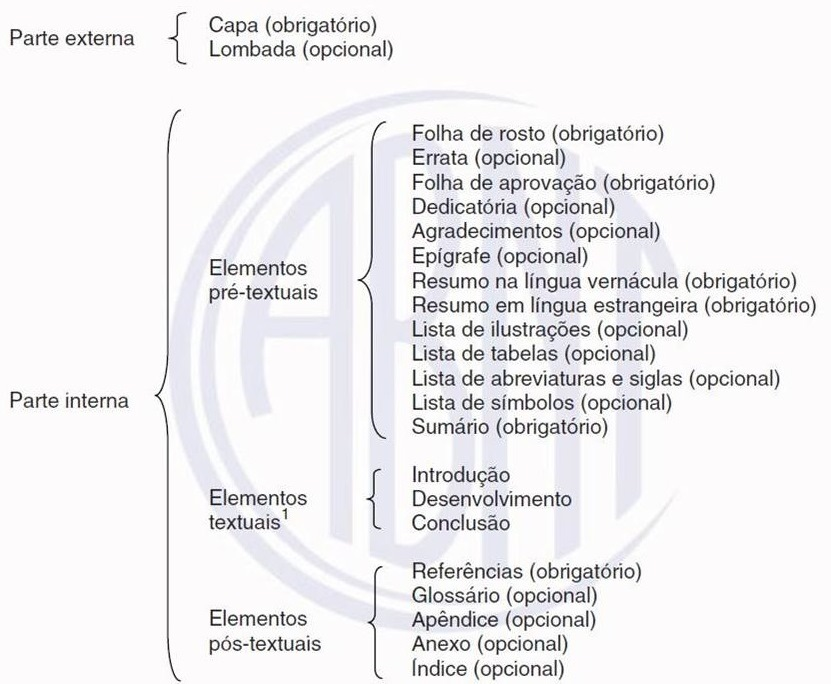
\includegraphics[scale=0.5]{USPSC-EstruturaTrabAcad.jpg}
	\end{center}
	\legend{Fonte: \citeonline{nbr14724}}
\end{figure}
		
O Pacote USPSC utiliza os seguintes arquivos para gerar o documento em formato PDF, mediante a compilação utilizando um dos editores \LaTeX\ :

\begin{alineas}	 
	\item USPSC.cls ou USPSC1.cls (classe USPSC); 
	\item Arquivos principais dos modelos: USPSC-modelo.tex  e  USPSC-TCC-modelo.tex;
	\item USPSC-unidades.tex;
	\item Arquivos pré-textuais: USPSC-pre-textual-UUUU.tex e USPSC-TCC-pre-textual-UUUU.tex;
	\item USPSC-fichacatalografica.tex;
	\item fichacatalografica.pdf;
	\item folhadeaprovacao.pdf;
	\item USPSC-Dedicatoria.tex;
	\item USPSC-Agradecimentos.tex;
	\item USPSC-Resumo.tex;
	\item USPSC-Abstract.tex;
	\item USPSC-Cap1-Introducao.tex;
	\item USPSC-Cap2-Desenvolvimento.tex;
	\item USPSC-Cap3-Citacoes.tex;
	\item USPSC-Cap4-Referencias.tex;
	\item USPSC-Cap5-Conclusao.tex;
	\item USPSC-Apendices.tex;
	\item USPSC-Anexos.tex;
	\item USPSC-AcentuacaoLaTeX.tex
	\item USPSC-LetrasGregas.tex
	\item USPSC-SimbolosUteis.tex
	\item USPSC-modelo-references.bib;
	
\end{alineas}	 

		
Para tese ou dissertação deverá ser utilizado o arquivo USPSC-modelo.tex, onde o autor deverá indicar a sigla da Unidade e a sigla do programa de pós-graduação que está vinculado, a exemplo dos comandos abaixo:
		
			\begin{verbatim}
				\siglaunidade{IQSC}
				\programa{MQOB}
			\end{verbatim}
			
Para o \textbf{Modelo para teses e dissertações em \LaTeX\ utilizando a classe USPSC} estão definidos os seguintes arquivos pré-textuais:
			
			\begin{alineas}	 
				\item USPSC-pre-textual-EESC.tex;
				\item USPSC-pre-textual-IAU.tex;
				\item USPSC-pre-textual-ICMC.tex;
				\item USPSC-pre-textual-IFSC.tex;
				\item USPSC-pre-textual-IQSC.tex.
			\end{alineas}
			
Para TCC deverá ser utilizado o arquivo USPSC-TCC-modelo.tex, onde o autor deverá indicar a \textbf{'sigla da Unidade'} + \textbf{'-TCC'} (Exemplo: EESC-TCC) e a sigla do curso de graduação que está vinculado, a exemplo dos comandos abaixo:
			
			\begin{verbatim}
			\siglaunidade{EESC-TCC}
			\programa{EAMB}
			\end{verbatim}
			
Atualmente estão disponíveis os dados pré-textuais apenas para a EESC:
			
			\begin{alineas}	 
				\item USPSC-TCC-pre-textual-EESC.tex;
			\end{alineas}
			
Assim que forem estabelecidos os padrões para as demais Unidades do Campus USP de São Carlos serão incluídos os demais arquivos.
			
			
É necessário consultar as siglas estabelecidas para os cursos e programas de pós-graduação da Unidade de vínculo \textbf{(APÊNDICES A-G)} ou nas planilhas \textbf{USPSC-TCC-Siglas estabelecidas para as Graduações por Unidade.xlsx} e \textbf{USPSC-Siglas estabelecidas para os programas de pós-graduação por Unidade.xlsx}, para utilizar corretamente os dados dados pre-textuais. 

Os arquivos com dados pre-textuais estão nominados como USPSC-pre-textual-UUUU.tex ou USPSC-TCC-pre-textual-UUUU.tex, onde UUUU é a sigla da Unidade. Inicialmente estão disponibilizados apenas os pré-textuais das Unidades do Campus USP de São Carlos.
			
Foram definido os arquivos USPSC-pre-textual-OUTRO.tex e USPSC-TCC-pre-textual-OUTRO.tex que serão executados quando uma das siglas for diferente das explicitadas para as Unidades, os cursos ou programas de Pós-Graduação, quando o preâmbulo será iniciado por "Dissertação/Tese"   ou por "Monografia apresentada ao Curso de Engenharia (?)", mostrando que o autor deverá rever as siglas utilizadas.

Através do comando \verb+ %% USPSC-unidadesTCC.tex
% Camando para definição do programa de Pós-Graduação, Especialidade do Título e Instituição - 21/09/2015
\newcommand{\siglaunidade}[1]{


% EESC-TCC ==========================================================================
    \ifthenelse{\equal{#1}{EESC-TCC}}{
     			%% USPSC-pre-textual-EESC.tex
%% Camandos para defini��o do tipo de documento (tese ou disserta��o), �rea de concentra��o, op��o, pre�mbulo, titula��o 
%% referentes aos Programas de P�s-Gradua��o
\instituicao{Escola de Engenharia de S\~ao Carlos, Universidade de S\~ao Paulo}
\unidade{ESCOLA DE ENGENHARIA DE S\~AO CARLOS}
\unidademin{Escola de Engenharia de S\~ao Carlos}
\universidademin{Universidade de S\~ao Paulo}
% A EESC n�o inclui a nota "Vers�o original", portanto o comando abaixo n�o tem a mensagem entre {}
\notafolharosto{ }
%Para a vers�o corrigida tire a % do comando/declara��o abaixo e inclua uma % antes do comando acima
%\notafolharosto{VERS\~AO CORRIGIDA}
% ---
% dados complementares para CAPA e FOLHA DE ROSTO
% ---
\universidade{UNIVERSIDADE DE S\~AO PAULO}
\titulo{Modelo para TCC em \LaTeX\ utilizando a classe USPSC para a EESC}
\titleabstract{Model for TCC in \LaTeX\ using the USPSC class to the EESC}
\autor{Jos\'e da Silva}
\autorficha{Silva, Jos\'e da}
\autorabr{SILVA, J.}

\cutter{S856m}
% Para gerar a ficha catalogr�fica sem o C�digo Cutter, basta 
% incluir uma % na linha acima e tirar a % da linha abaixo
%\cutter{ }

\local{S\~ao Carlos}
\data{2017}
% Quando for Orientador, basta incluir uma % antes do comando abaixo
\renewcommand{\orientadorname}{Orientadora:}
% Quando for Coorientadora, basta tirar a % do comando abaixo
%\newcommand{\coorientadorname}{Coorientador:}
\orientador{Profa. Dra. Elisa Gon\c{c}alves Rodrigues}
%\orientadorcorpoficha{orientadora Elisa Gon\c{c}alves Rodrigues}
%\orientadorficha{Rodrigues, Elisa Gon\c{c}alves, orient}
%Se houver co-orientador, inclua % antes das duas linhas (antes dos comandos \orientadorcorpoficha e \orientadorficha) 
%          e tire a % antes dos 3 comandos abaixo
\coorientador{Prof. Dr. Jo\~ao Alves Serqueira}
\orientadorcorpoficha{orientadora Elisa Gon\c{c}alves Rodrigues ;  co-orientador Jo\~ao Alves Serqueira}
\orientadorficha{Rodrigues, Elisa Gon\c{c}alves, orient. II. Serqueira, Jo\~ao Alves, co-orient}

\notaautorizacao{AUTORIZO A REPRODU\c{C}\~AO E DIVULGA\c{C}\~AO TOTAL OU PARCIAL DESTE TRABALHO, POR QUALQUER MEIO CONVENCIONAL OU ELETR\^ONICO PARA FINS DE ESTUDO E PESQUISA, DESDE QUE CITADA A FONTE.}
\notabib{~  ~}

\newcommand{\programa}[1]{


% EAMB ==========================================================================
    \ifthenelse{\equal{#1}{EAMB}}{
     	\tipotrabalho{Monografia (Trabalho de Conclus\~ao de Curso)}
        %\area{Nome da �rea}
		%\opcao{Nome da Op��o}
        % O preambulo deve conter o tipo do trabalho, o objetivo, 
		% o nome da institui��o, a �rea de concentra��o e op��o quando houver
		\preambulo{Monografia apresentada ao Curso de Engenharia Ambiental, da Escola de Engenharia de S\~ao Carlos da Universidade de S\~ao Paulo, como parte dos requisitos para obten\c{c}\~ao do t\'itulo de Engenheiro Ambiental.}
		\notaficha{Monografia (Gradua\c{c}\~ao em Engenharia Ambiental)}
    }{
% EAER ===========================================================================
        \ifthenelse{\equal{#1}{EAER}}{
	        \tipotrabalho{Monografia (Trabalho de Conclus\~ao de Curso)}
	        %\area{Nome da �rea}
			%\opcao{Nome da Op��o}
		    % O preambulo deve conter o tipo do trabalho, o objetivo, 
			% o nome da institui��o, a �rea de concentra��o e op��o quando houver
			\preambulo{Monografia apresentada ao Curso de Engenharia Aeron\'autica, da Escola de Engenharia de S\~ao Carlos da Universidade de S\~ao Paulo, como parte dos requisitos para obten\c{c}\~ao do t\'itulo de Engenheiro Aeron\'autico.}
			\notaficha{Monografia (Gradua\c{c}\~ao em Engenharia Aeron\'autica)}
        }{
% ECIV =======================================================================
    \ifthenelse{\equal{#1}{ECIV}}{
     	\tipotrabalho{Monografia (Trabalho de Conclus\~ao de Curso)}
     	%\area{Nome da �rea}
     	%\opcao{Nome da Op��o}
        % O preambulo deve conter o tipo do trabalho, o objetivo, 
		% o nome da institui��o, a �rea de concentra��o e op��o quando houver
		\preambulo{Monografia apresentada ao Curso de Engenharia Civil, da Escola de Engenharia de S\~ao Carlos da Universidade de S\~ao Paulo, como parte dos requisitos para obten\c{c}\~ao do t\'itulo de Engenheiro Civil.}
		\notaficha{Monografia (Gradua\c{c}\~ao em Engenharia Civil)}
    }{
% ECOM ===========================================================================
        \ifthenelse{\equal{#1}{ECOM}}{
			\tipotrabalho{Monografia (Trabalho de Conclus\~ao de Curso)}
			%\area{Nome da �rea}
			%\opcao{Nome da Op��o}
			% O preambulo deve conter o tipo do trabalho, o objetivo, 
			% o nome da institui��o, a �rea de concentra��o e op��o quando houver
			\preambulo{Monografia apresentada ao Curso de Engenharia de Computa\c{c}\~ao, da Escola de Engenharia de S\~ao Carlos e Instituto de Ci\^encias Matem\'aticas e de Computa\c{c}\~ao da Universidade de S\~ao Paulo, como parte dos requisitos para obten\c{c}\~ao do t\'itulo de Engenheiro de Computa\c{c}\~ao.}
			\notaficha{Monografia (Gradua\c{c}\~ao em Engenharia de Computa\c{c}\~ao)}
        }{
% EELT ==========================================================================
    \ifthenelse{\equal{#1}{EELT}}{
     	\tipotrabalho{Monografia (Trabalho de Conclus\~ao de Curso)}
     	%\area{Nome da �rea}
     	%\opcao{Nome da Op��o}
     	% O preambulo deve conter o tipo do trabalho, o objetivo, 
     	% o nome da institui��o, a �rea de concentra��o e op��o quando houver
     	\preambulo{Monografia apresentada ao Curso de Engenharia El\'etrica com \^Enfase em Eletr\^onica, da Escola de Engenharia de S\~ao Carlos da Universidade de S\~ao Paulo, como parte dos requisitos para obten\c{c}\~ao do t\'itulo de Engenheiro Eletricista.}
     	\notaficha{Monografia (Gradua\c{c}\~ao em Engenharia El\'etrica com \^Enfase em Eletr\^onica)}
    }{
% EELS ===========================================================================
        \ifthenelse{\equal{#1}{EELS}}{
	        \tipotrabalho{Monografia (Trabalho de Conclus\~ao de Curso)}
	        %\area{Nome da �rea}
	        %\opcao{Nome da Op��o}
	        % O preambulo deve conter o tipo do trabalho, o objetivo, 
	        % o nome da institui��o, a �rea de concentra��o e op��o quando houver
	        \preambulo{Monografia apresentada ao Curso de Curso de Engenharia El\'etrica com \^Enfase em Sistemas de Energia e Automa\c{c}\~ao, da Escola de Engenharia de S\~ao Carlos da Universidade de S\~ao Paulo, como parte dos requisitos para obten\c{c}\~ao do t\'itulo de Engenheiro Eletricista.}
	        \notaficha{Monografia (Gradua\c{c}\~ao em Engenharia El\'etrica com \^Enfase Sistemas de Energia e Automa\c{c}\~ao)}
        }{			
% EMAT ==========================================================================
    \ifthenelse{\equal{#1}{EMAT}}{
     	\tipotrabalho{Monografia (Trabalho de Conclus\~ao de Curso)}
     	%\area{Nome da �rea}
     	%\opcao{Nome da Op��o}
     	% O preambulo deve conter o tipo do trabalho, o objetivo, 
     	% o nome da institui��o, a �rea de concentra��o e op��o quando houver
     	\preambulo{Monografia apresentada ao Curso de Engenharia de Materiais e Manufatura, da Escola de Engenharia de S\~ao Carlos da Universidade de S\~ao Paulo, como parte dos requisitos para obten\c{c}\~ao do t\'itulo de Engenheiro de Materiais e de Manufatura.}
     	\notaficha{Monografia (Gradua\c{c}\~ao em Engenharia de Materiais e Manufatura)}
    }{
% EMEC ===========================================================================
        \ifthenelse{\equal{#1}{EMEC}}{
	        \tipotrabalho{Monografia (Trabalho de Conclus\~ao de Curso)}
	        %\area{Nome da �rea}
	        %\opcao{Nome da Op��o}
	        % O preambulo deve conter o tipo do trabalho, o objetivo, 
	        % o nome da institui��o, a �rea de concentra��o e op��o quando houver
	        \preambulo{Monografia apresentada ao Curso de Engenharia Mec\^anica, da Escola de Engenharia de S\~ao Carlos da Universidade de S\~ao Paulo, como parte dos requisitos para obten\c{c}\~ao do t\'itulo de Engenheiro Mec\^anico.}
	        \notaficha{Monografia (Gradua\c{c}\~ao em Engenharia Mec\^anica)}
         }{			
% EMET ===========================================================================
         \ifthenelse{\equal{#1}{EMET}}{
         	\tipotrabalho{Monografia (Trabalho de Conclus\~ao de Curso)}
         	%\area{Nome da �rea}
         	%\opcao{Nome da Op��o}
         	% O preambulo deve conter o tipo do trabalho, o objetivo, 
         	% o nome da institui��o, a �rea de concentra��o e op��o quando houver
         	\preambulo{Monografia apresentada ao Curso de Engenharia Mecatr\^onica, da Escola de Engenharia de S\~ao Carlos da Universidade de S\~ao Paulo, como parte dos requisitos para obten\c{c}\~ao do t\'itulo de Engenheiro Mecatr\^onico.}
         	\notaficha{Monografia (Gradua\c{c}\~ao em Engenharia Mecatr\^onica)}
         }{		
% EPRO ===========================================================================
\ifthenelse{\equal{#1}{EPRO}}{
	\tipotrabalho{Monografia (Trabalho de Conclus\~ao de Curso)}
	%\area{Nome da �rea}
	%\opcao{Nome da Op��o}
	% O preambulo deve conter o tipo do trabalho, o objetivo, 
	% o nome da institui��o, a �rea de concentra��o e op��o quando houver
	\preambulo{Monografia apresentada ao Curso de Engenharia de Produ\c{c}\~ao, da Escola de Engenharia de S\~ao Carlos da Universidade de S\~ao Paulo, como parte dos requisitos para obten\c{c}\~ao do t\'itulo de Engenheiro de Produ\c{c}\~ao.}
	\notaficha{Monografia (Gradua\c{c}\~ao em Engenharia de Produ\c{c}\~a)}
}{		         	
% Outros
	\tipotrabalho{Monografia (Trabalho de Conclus\~ao de Curso)}
	%\area{Nome da �rea}
	%\opcao{Nome da Op��o}
	% O preambulo deve conter o tipo do trabalho, o objetivo, 
	% o nome da institui��o, a �rea de concentra��o e op��o quando houver
	\preambulo{Monografia apresentada ao Curso de Engenharia (?), da Escola de Engenharia de S\~ao Carlos da Universidade de S\~ao Paulo, como parte dos requisitos para obten\c{c}\~ao do t\'itulo de Engenheiro (?).}
	\notaficha{Monografia (Gradua\c{c}\~ao em Engenharia (?))}		
        }}}}}}}}}}}
        				
% ---
    }{
% EESC ==========================================================================
	\ifthenelse{\equal{#1}{EESC}}{
	%% USPSC-pre-textual-EESC.tex
%% Camandos para defini��o do tipo de documento (tese ou disserta��o), �rea de concentra��o, op��o, pre�mbulo, titula��o 
%% referentes aos Programas de P�s-Gradua��o
\instituicao{S\~ao Carlos School of Engineering, University of S\~ao Paulo}
\unidade{S\~AO CARLOS SCHOOL OF ENGINEERING}
\unidademin{S\~ao Carlos School of Engineering}
\universidademin{University of S\~ao Paulo}
% A EESC n�o inclui a nota "Vers�o original", portanto o comando abaixo n�o tem a mensagem entre {}
%\notafolharosto{ }
%Para a vers�o corrigida tire a % do comando/declara��o abaixo e inclua uma % antes do comando acima
\notafolharosto{FINAL VERSION}
% ---
% dados complementares para CAPA e FOLHA DE ROSTO
% ---
\universidade{UNIVERSITY OF S\~AO PAULO}
\titulo{Development of Software for Parameter Estimation and its Application on Wind Power Plant Equivalent Model}
\titleabstract{Desenvolvimento de Software para Estima\c{c}\~ao de Par\^ametros e sua aplica\c{c}\~ao em Modelo Equivalente de Parques E\'olicos}
\autor{Gabriel Jos\'e Negrelli Gomes}
\autorficha{Gomes, Gabriel Jos\'e Negrelli}
\autorabr{GOMES, G. J. N.}

\cutter{G633d}
% Para gerar a ficha catalogr�fica sem o C�digo Cutter, basta 
% incluir uma % na linha acima e tirar a % da linha abaixo
%\cutter{ }

\local{S\~ao Carlos}
\data{2020}
% Quando for Orientador, basta incluir uma % antes do comando abaixo
\renewcommand{\orientadorname}{Advisor:}
% Quando for Coorientadora, basta tirar a % utilizar o comando abaixo
%\newcommand{\coorientadorname}{Coorientador:}
\orientador{Prof. Dr. Elmer Pablo Tito Cari}
\orientadorcorpoficha{advisor Elmer Pablo Tito Cari}
\orientadorficha{Cari, Elmer Pablo Tito, advisor}
%Se houver co-orientador, inclua % antes das duas linhas (antes dos comandos \orientadorcorpoficha e \orientadorficha) 
%          e tire a % antes dos 3 comandos abaixo
%\coorientador{Prof. Dr. Jo\~ao Alves Serqueira}
%\orientadorcorpoficha{orientadora Elisa Gon\c{c}alves Rodrigues ;  co-orientador Jo\~ao Alves Serqueira}
%\orientadorficha{Rodrigues, Elisa Gon\c{c}alves, orient. II. Serqueira, Jo\~ao Alves, co-orient}

\notaautorizacao{I HEREBY AUTHORIZE THE TOTAL OR PARTIAL REPRODUCTION OF THIS WORK BY ANY CONVENTIONAL OR ELECTRONIC MEANS, FOR RESEARCH PURPOSES, PROVIDED THE SOURCE IS PROPERLY ACKNOWLEDGED.}
\notabib{~  ~}

\newcommand{\programa}[1]{

% DCEA ==========================================================================
    \ifthenelse{\equal{#1}{DCEA}}{
     	\tipotrabalho{Tese (Doutorado)}
        \area{Ci\^encias da Engenharia Ambiental}
		%\opcao{Nome da Op��o}
        % O preambulo deve conter o tipo do trabalho, o objetivo, 
		% o nome da institui��o, a �rea de concentra��o e op��o quando houver
		\preambulo{Tese apresentada \`a Escola de Engenharia de S\~ao Carlos da Universidade de S\~ao Paulo, para obten\c{c}\~ao do t\'itulo de Doutor em Ci\^encias - Programa de P\'os-Gradua\c{c}\~ao em Ci\^encias da Engenharia Ambiental.}
		\notaficha{Tese (Doutorado) - Programa de P\'os-Gradua\c{c}\~ao e \'Area de Concentra\c{c}\~ao em Ci\^encias da Engenharia Ambiental}
    }{
% MCEA ===========================================================================
        \ifthenelse{\equal{#1}{MCEA}}{
	        \tipotrabalho{Disserta\c{c}\~ao (Mestrado)}
	        \area{Ci\^encias da Engenharia Ambiental}
			%\opcao{Nome da Op��o}
		    % O preambulo deve conter o tipo do trabalho, o objetivo, 
			% o nome da institui��o, a �rea de concentra��o e op��o quando houver
			\preambulo{Disserta\c{c}\~ao apresentada \`a Escola de Engenharia de S\~ao Carlos da Universidade de S\~ao Paulo, para obten\c{c}\~ao do t\'itulo de Mestre em Ci\^encias - Programa de P\'os-Gradua\c{c}\~ao em Ci\^encias da Engenharia Ambiental.}
			\notaficha{Disserta\c{c}\~ao (Mestrado) - Programa de P\'os-Gradua\c{c}\~ao e \'Area de Concentra\c{c}\~ao em Ci\^encias da Engenharia Ambiental}
        }{
% DEE =======================================================================
    \ifthenelse{\equal{#1}{DEE}}{
     	\tipotrabalho{Tese (Doutorado)}
        \area{Estruturas}
		%\opcao{Nome da Op��o}
        % O preambulo deve conter o tipo do trabalho, o objetivo, 
		% o nome da institui��o, a �rea de concentra��o e op��o quando houver
		\preambulo{Tese apresentada \`a Escola de Engenharia de S\~ao Carlos da Universidade de S\~ao Paulo, para obten\c{c}\~ao do t\'itulo de Doutor em Ci\^encias - Programa de P\'os-Gradua\c{c}\~ao em Engenharia Civil (Engenharia de Estruturas).}
		\notaficha{Tese (Doutorado) - Programa de P\'os-Gradua\c{c}\~ao em Engenharia Civil (Engenharia de Estruturas) e \'Area de Concentra\c{c}\~ao em Estruturas}
    }{
% MEE ===========================================================================
        \ifthenelse{\equal{#1}{MEE}}{
			\tipotrabalho{Disserta\c{c}\~ao (Mestrado)}
			\area{Estruturas}
			%\opcao{Nome da Op��o}
	        % O preambulo deve conter o tipo do trabalho, o objetivo, 
			% o nome da institui��o, a �rea de concentra��o e op��o quando houver
			\preambulo{Disserta\c{c}\~ao apresentada \`a Escola de Engenharia de S\~ao Carlos da Universidade de S\~ao Paulo, para obten\c{c}\~ao do t\'itulo de Mestre em Ci\^encias - Programa de P\'os-Gradua\c{c}\~ao em Engenharia Civil (Engenharia de Estruturas).}
			\notaficha{Disserta\c{c}\~ao (Mestrado) - Programa de P\'os-Gradua\c{c}\~ao em Engenharia Civil (Engenharia de Estruturas) e \'Area de Concentra\c{c}\~ao em Estruturas}
        }{
% DEPP ==========================================================================
    \ifthenelse{\equal{#1}{DEPP}}{
     	\tipotrabalho{Tese (Doutorado)}
        \area{Processos e Gest\~ao de Opera\c{c}\~oes}
		%\opcao{Nome da Op��o}
        % O preambulo deve conter o tipo do trabalho, o objetivo, 
		% o nome da institui��o, a �rea de concentra��o e op��o quando houver
		\preambulo{Tese apresentada \`a Escola de Engenharia de S\~ao Carlos da Universidade de S\~ao Paulo, para obten\c{c}\~ao do t\'itulo de Doutor em Ci\^encias - Programa de P\'os-Gradua\c{c}\~ao em Engenharia de Produ\c{c}\~ao.}
		\notaficha{Tese (Doutorado) - Programa de P\'os-Gradua\c{c}\~ao em Engenharia de Produ\c{c}\~ao e \'Area de Concentra\c{c}\~ao em Processos e Gest\~ao de Opera\c{c}\~oes}
    }{
% MEPP ===========================================================================
        \ifthenelse{\equal{#1}{MEPP}}{
	        \tipotrabalho{Disserta\c{c}\~ao (Mestrado)}
	        \area{Processos e Gest\~ao de Opera\c{c}\~oes}
			%\opcao{Nome da Op��o}
	        % O preambulo deve conter o tipo do trabalho, o objetivo, 
			% o nome da institui��o, a �rea de concentra��o e op��o quando houver
			\preambulo{Disserta\c{c}\~ao apresentada \`a Escola de Engenharia de S\~ao Carlos da Universidade de S\~ao Paulo, para obten\c{c}\~ao do t\'itulo de Mestre em Ci\^encias - Programa de P\'os-Gradua\c{c}\~ao em Engenharia de Produ\c{c}\~ao.}
			\notaficha{Disserta\c{c}\~ao (Mestrado) - Programa de P\'os-Gradua\c{c}\~ao em Engenharia de Produ\c{c}\~ao e \'Area de Concentra\c{c}\~ao em Processos e Gest\~ao de Opera\c{c}\~oes}
        }{			
% DEPE ==========================================================================
    \ifthenelse{\equal{#1}{DEPE}}{
     	\tipotrabalho{Tese (Doutorado)}
        \area{Economia, Organiza\c{c}\~oes e Gest\~ao do Conhecimento}
		%\opcao{Nome da Op��o}
        % O preambulo deve conter o tipo do trabalho, o objetivo, 
		% o nome da institui��o, a �rea de concentra��o e op��o quando houver
		\preambulo{Tese apresentada \`a Escola de Engenharia de S\~ao Carlos da Universidade de S\~ao Paulo, para obten\c{c}\~ao do t\'itulo de Doutor em Ci\^encias - Programa de P\'os-Gradua\c{c}\~ao em Engenharia de Produ\c{c}\~ao.}
		\notaficha{Tese (Doutorado) - Programa de P\'os-Gradua\c{c}\~ao em Engenharia de Produ\c{c}\~ao e \'Area de Concentra\c{c}\~ao em Economia, Organiza\c{c}\~oes e Gest\~ao do Conhecimento}
    }{
% MEPE ===========================================================================
        \ifthenelse{\equal{#1}{MEPE}}{
	        \tipotrabalho{Disserta\c{c}\~ao (Mestrado)}
	        \area{Economia, Organiza\c{c}\~oes e Gest\~ao do Conhecimento}
			%\opcao{Nome da Op��o}
	        % O preambulo deve conter o tipo do trabalho, o objetivo, 
			% o nome da institui��o, a �rea de concentra��o e op��o quando houver
			\preambulo{Disserta\c{c}\~ao apresentada \`a Escola de Engenharia de S\~ao Carlos da Universidade de S\~ao Paulo, para obten\c{c}\~ao do t\'itulo de Mestre em Ci\^encias - Programa de P\'os-Gradua\c{c}\~ao em Engenharia de Produ\c{c}\~ao.}
			\notaficha{Disserta\c{c}\~ao (Mestrado) - Programa de P\'os-Gradua\c{c}\~ao em Engenharia de Produ\c{c}\~ao e \'Area de Concentra\c{c}\~ao em Economia, Organiza\c{c}\~oes e Gest\~ao do Conhecimento}
         }{			
% DETI ==========================================================================
    \ifthenelse{\equal{#1}{DETI}}{
     	\tipotrabalho{Tese (Doutorado)}
        \area{Infraestrutura de Transportes}
		%\opcao{Nome da Op��o}
        % O preambulo deve conter o tipo do trabalho, o objetivo, 
		% o nome da institui��o, a �rea de concentra��o e op��o quando houver
		\preambulo{Tese apresentada \`a Escola de Engenharia de S\~ao Carlos da Universidade de S\~ao Paulo, para obten\c{c}\~ao do t\'itulo de Doutor em Ci\^encias - Programa de P\'os-Gradua\c{c}\~ao em Engenharia de Transportes.}
		\notaficha{Tese (Doutorado) - Programa de P\'os-Gradua\c{c}\~ao em Engenharia de Transportes e \'Area de Concentra\c{c}\~ao em Infraestrutura de Transportes}
    }{
% METI ===========================================================================
        \ifthenelse{\equal{#1}{METI}}{
	        \tipotrabalho{Disserta\c{c}\~ao (Mestrado)}
	        \area{Infraestrutura de Transportes}
			%\opcao{Nome da Op��o}
	        % O preambulo deve conter o tipo do trabalho, o objetivo, 
			% o nome da institui��o, a �rea de concentra��o e op��o quando houver
			\preambulo{Disserta\c{c}\~ao apresentada \`a Escola de Engenharia de S\~ao Carlos da Universidade de S\~ao Paulo, para obten\c{c}\~ao do t\'itulo de Mestre em Ci\^encias - Programa de P\'os-Gradua\c{c}\~ao em Engenharia de Transportes.}
			\notaficha{Disserta\c{c}\~ao (Mestrado) - Programa de P\'os-Gradua\c{c}\~ao em Engenharia de Transportes e \'Area de Concentra\c{c}\~ao em Infraestrutura de Transportes}
         }{	   			
% DETT ==========================================================================
    \ifthenelse{\equal{#1}{DETT}}{
     	\tipotrabalho{Tese (Doutorado)}
        \area{Transportes}
		%\opcao{Nome da Op��o}
        % O preambulo deve conter o tipo do trabalho, o objetivo, 
		% o nome da institui��o, a �rea de concentra��o e op��o quando houver
		\preambulo{Tese apresentada \`a Escola de Engenharia de S\~ao Carlos da Universidade de S\~ao Paulo, para obten\c{c}\~ao do t\'itulo de Doutor em Ci\^encias - Programa de P\'os-Gradua\c{c}\~ao em Engenharia de Transportes.}
		\notaficha{Tese (Doutorado) - Programa de P\'os-Gradua\c{c}\~ao em Engenharia de Transportes e \'Area de Concentra\c{c}\~ao em Transportes}
    }{
% METT ===========================================================================
        \ifthenelse{\equal{#1}{METT}}{
	        \tipotrabalho{Disserta\c{c}\~ao (Mestrado)}
	        \area{Transportes}
			%\opcao{Nome da Op��o}
		    % O preambulo deve conter o tipo do trabalho, o objetivo, 
			% o nome da institui��o, a �rea de concentra��o e op��o quando houver
			\preambulo{Disserta\c{c}\~ao apresentada \`a Escola de Engenharia de S\~ao Carlos da Universidade de S\~ao Paulo, para obten\c{c}\~ao do t\'itulo de Mestre em Ci\^encias - Programa de P\'os-Gradua\c{c}\~ao em Engenharia de Transportes.}
			\notaficha{Disserta\c{c}\~ao (Mestrado) - Programa de P\'os-Gradua\c{c}\~ao em Engenharia de Transportes e \'Area de Concentra\c{c}\~ao em Transportes}
         }{	  				
% DETP ==========================================================================
    \ifthenelse{\equal{#1}{DETP}}{
     	\tipotrabalho{Tese (Doutorado)}
        \area{Planejamento e Opera\c{c}\~ao de Sistemas de Transporte}
		%\opcao{Nome da Op��o}
        % O preambulo deve conter o tipo do trabalho, o objetivo, 
		% o nome da institui��o, a �rea de concentra��o e op��o quando houver
		\preambulo{Tese apresentada \`a Escola de Engenharia de S\~ao Carlos da Universidade de S\~ao Paulo, para obten\c{c}\~ao do t\'itulo de Doutor em Ci\^encias - Programa de P\'os-Gradua\c{c}\~ao em Engenharia de Transportes.}
		\notaficha{Tese (Doutorado) - Programa de P\'os-Gradua\c{c}\~ao em Engenharia de Transportes e \'Area de Concentra\c{c}\~ao em Planejamento e Opera\c{c}\~ao de Sistemas de Transporte}
    }{
% METP ===========================================================================
        \ifthenelse{\equal{#1}{METP}}{
	        \tipotrabalho{Disserta\c{c}\~ao (Mestrado)}
	        \area{Planejamento e Opera\c{c}\~ao de Sistemas de Transporte}
			%\opcao{Nome da Op��o}
		    % O preambulo deve conter o tipo do trabalho, o objetivo, 
			% o nome da institui��o, a �rea de concentra��o e op��o quando houver
			\preambulo{Disserta\c{c}\~ao apresentada \`a Escola de Engenharia de S\~ao Carlos da Universidade de S\~ao Paulo, para obten\c{c}\~ao do t\'itulo de Mestre em Ci\^encias - Programa de P\'os-Gradua\c{c}\~ao em Engenharia de Transportes.}
			\notaficha{Disserta\c{c}\~ao (Mestrado) - Programa de P\'os-Gradua\c{c}\~ao em Engenharia de Transportes e \'Area de Concentra\c{c}\~ao em Planejamento e Opera\c{c}\~ao de Sistemas de Transporte}
         }{	    
% DEEP ==========================================================================
    \ifthenelse{\equal{#1}{DEEP}}{
     	\tipotrabalho{Tese (Doutorado)}
        \area{Processamento de Sinais e Instrumenta\c{c}\~ao}
		%\opcao{Nome da Op��o}
		% O preambulo deve conter o tipo do trabalho, o objetivo, 
		% o nome da institui��o, a �rea de concentra��o e op��o quando houver
		\preambulo{Tese apresentada \`a Escola de Engenharia de S\~ao Carlos da Universidade de S\~ao Paulo, para obten\c{c}\~ao do t\'itulo de Doutor em Ci\^encias - Programa de P\'os-Gradua\c{c}\~ao em Engenharia El\'etrica.}
		\notaficha{Tese (Doutorado) - Programa de P\'os-Gradua\c{c}\~ao em Engenharia El\'etrica e \'Area de Concentra\c{c}\~ao em Processamento de Sinais e Instrumenta\c{c}\~ao}
    }{
% MEEP ===========================================================================
        \ifthenelse{\equal{#1}{MEEP}}{
	        \tipotrabalho{Disserta\c{c}\~ao (Mestrado)}
	        \area{Processamento de Sinais e Instrumenta\c{c}\~ao}
			%\opcao{Nome da Op��o}
	        % O preambulo deve conter o tipo do trabalho, o objetivo, 
			% o nome da institui��o, a �rea de concentra��o e op��o quando houver
			\preambulo{Disserta\c{c}\~ao apresentada \`a Escola de Engenharia de S\~ao Carlos da Universidade de S\~ao Paulo, para obten\c{c}\~ao do t\'itulo de Mestre em Ci\^encias - Programa de P\'os-Gradua\c{c}\~ao em Engenharia El\'etrica.}
			\notaficha{Disserta\c{c}\~ao (Mestrado) - Programa de P\'os-Gradua\c{c}\~ao em Engenharia El\'etrica e \'Area de Concentra\c{c}\~ao em Processamento de Sinais e Instrumenta\c{c}\~ao}
         }{	  
% DEED ==========================================================================
    \ifthenelse{\equal{#1}{DEED}}{
     	\tipotrabalho{Tese (Doutorado)}
        \area{Sistemas Din\^amicos}
		%\opcao{Nome da Op��o}
        % O preambulo deve conter o tipo do trabalho, o objetivo, 
		% o nome da institui��o, a �rea de concentra��o e op��o quando houver
		\preambulo{Tese apresentada \`a Escola de Engenharia de S\~ao Carlos da Universidade de S\~ao Paulo, para obten\c{c}\~ao do t\'itulo de Doutor em Ci\^encias - Programa de P\'os-Gradua\c{c}\~ao em Engenharia El\'etrica.}
		\notaficha{Tese (Doutorado) - Programa de P\'os-Gradua\c{c}\~ao em Engenharia El\'etrica e \'Area de Concentra\c{c}\~ao em Sistemas Din\^amicos}
    }{
% MEED ===========================================================================
        \ifthenelse{\equal{#1}{MEED}}{
	        \tipotrabalho{Disserta\c{c}\~ao (Mestrado)}
	        \area{Sistemas Din\^amicos}
			%\opcao{Nome da Op��o}
	        % O preambulo deve conter o tipo do trabalho, o objetivo, 
			% o nome da institui��o, a �rea de concentra��o e op��o quando houver
			\preambulo{Disserta\c{c}\~ao apresentada \`a Escola de Engenharia de S\~ao Carlos da Universidade de S\~ao Paulo, para obten\c{c}\~ao do t\'itulo de Mestre em Ci\^encias - Programa de P\'os-Gradua\c{c}\~ao em Engenharia El\'etrica.}
			\notaficha{Disserta\c{c}\~ao (Mestrado) - Programa de P\'os-Gradua\c{c}\~ao em Engenharia El\'etrica e \'Area de Concentra\c{c}\~ao em Sistemas Din\^amicos}
         }{	  
% DEEE ==========================================================================
    \ifthenelse{\equal{#1}{DEEE}}{
     	\tipotrabalho{Tese (Doutorado)}
        \area{Sistemas El\'etricos de Pot\^encia}
		%\opcao{Nome da Op��o}
        % O preambulo deve conter o tipo do trabalho, o objetivo, 
		% o nome da institui��o, a �rea de concentra��o e op��o quando houver
		\preambulo{Tese apresentada \`a Escola de Engenharia de S\~ao Carlos da Universidade de S\~ao Paulo, para obten\c{c}\~ao do t\'itulo de Doutor em Ci\^encias - Programa de P\'os-Gradua\c{c}\~ao em Engenharia El\'etrica.}
		\notaficha{Tese (Doutorado) - Programa de P\'os-Gradua\c{c}\~ao em Engenharia El\'etrica e \'Area de Concentra\c{c}\~ao em Sistemas El\'etricos de Pot\^encia}
    }{
% MEEE ===========================================================================
        \ifthenelse{\equal{#1}{MEEE}}{
        \tipotrabalho{Dissertation (Masters)}
        \area{Electrical Power Systems}
		%\opcao{Nome da Op��o}
        % O preambulo deve conter o tipo do trabalho, o objetivo, 
		% o nome da institui��o, a �rea de concentra��o e op��o quando houver
		\preambulo{Dissertation presented to the S\~ao Carlos School of Engineering at the University of S\~ao Paulo in fulfillment of the requirements for the degree of Master of Science in Electrical Engineering.}
		\notaficha{Dissertation (Masters) - Post-Graduation Program in Electrical Engineering, Electrical Power Systems Area}
         }{	  
% DEET ==========================================================================
    \ifthenelse{\equal{#1}{DEET}}{
     	\tipotrabalho{Tese (Doutorado)}
        \area{Telecomunica\c{c}\~oes}
		%\opcao{Nome da Op��o}
        % O preambulo deve conter o tipo do trabalho, o objetivo, 
		% o nome da institui��o, a �rea de concentra��o e op��o quando houver
		\preambulo{Tese apresentada \`a Escola de Engenharia de S\~ao Carlos da Universidade de S\~ao Paulo, para obten\c{c}\~ao do t\'itulo de Doutor em Ci\^encias - Programa de P\'os-Gradua\c{c}\~ao em Engenharia El\'etrica.}
		\notaficha{Tese (Doutorado) - Programa de P\'os-Gradua\c{c}\~ao em Engenharia El\'etrica e \'Area de Concentra\c{c}\~ao em Telecomunica\c{c}\~oes}
    }{
% MEET ===========================================================================
        \ifthenelse{\equal{#1}{MEET}}{
	        \tipotrabalho{Disserta\c{c}\~ao (Mestrado)}
	        \area{Telecomunica\c{c}\~oes}
			%\opcao{Nome da Op��o}
	        % O preambulo deve conter o tipo do trabalho, o objetivo, 
			% o nome da institui��o, a �rea de concentra��o e op��o quando houver
			\preambulo{Disserta\c{c}\~ao apresentada \`a Escola de Engenharia de S\~ao Carlos da Universidade de S\~ao Paulo, para obten\c{c}\~ao do t\'itulo de Mestre em Ci\^encias - Programa de P\'os-Gradua\c{c}\~ao em Engenharia El\'etrica.}
			\notaficha{Disserta\c{c}\~ao (Mestrado) - Programa de P\'os-Gradua\c{c}\~ao em Engenharia El\'etrica e \'Area de Concentra\c{c}\~ao em Telecomunica\c{c}\~oes}
         }{	
% DEHS ==========================================================================
    \ifthenelse{\equal{#1}{DEHS}}{
     	\tipotrabalho{Tese (Doutorado)}
        \area{Hidr\'aulica e Saneamento}
		%\opcao{Nome da Op��o}
        % O preambulo deve conter o tipo do trabalho, o objetivo, 
		% o nome da institui��o, a �rea de concentra��o e op��o quando houver
		\preambulo{Tese apresentada \`a Escola de Engenharia de S\~ao Carlos da Universidade de S\~ao Paulo, para obten\c{c}\~ao do t\'itulo de Doutor em Ci\^encias - Programa de P\'os-Gradua\c{c}\~ao em Engenharia Hidr\'aulica e Saneamento.}
		\notaficha{Tese (Doutorado) - Programa de P\'os-Gradua\c{c}\~ao e \'Area de Concentra\c{c}\~ao em Engenharia Hidr\'aulica e Saneamento}
    }{
% MEHS ===========================================================================
        \ifthenelse{\equal{#1}{MEHS}}{
	        \tipotrabalho{Disserta\c{c}\~ao (Mestrado)}
	        \area{Hidr\'aulica e Saneamento}
			%\opcao{Nome da Op��o}
	        % O preambulo deve conter o tipo do trabalho, o objetivo, 
			% o nome da institui��o, a �rea de concentra��o e op��o quando houver
			\preambulo{Disserta\c{c}\~ao apresentada \`a Escola de Engenharia de S\~ao Carlos da Universidade de S\~ao Paulo, para obten\c{c}\~ao do t\'itulo de Mestre em Ci\^encias - Programa de P\'os-Gradua\c{c}\~ao em Hidr\'aulica e Saneamento.}
			\notaficha{Disserta\c{c}\~ao (Mestrado) - Programa de P\'os-Gradua\c{c}\~ao e \'Area de Concentra\c{c}\~ao em Engenharia Hidr\'aulica e Saneamento} 
         }{	
% DEMA ==========================================================================
    \ifthenelse{\equal{#1}{DEMA}}{
     	\tipotrabalho{Tese (Doutorado)}
        \area{Aeronaves}
		%\opcao{Nome da Op��o}
        % O preambulo deve conter o tipo do trabalho, o objetivo, 
		% o nome da institui��o, a �rea de concentra��o e op��o quando houver
		\preambulo{Tese apresentada \`a Escola de Engenharia de S\~ao Carlos da Universidade de S\~ao Paulo, para obten\c{c}\~ao do t\'itulo de Doutor em Ci\^encias - Programa de P\'os-Gradua\c{c}\~ao em Engenharia Mec\^anica.}
		\notaficha{Tese (Doutorado) - Programa de P\'os-Gradua\c{c}\~ao em Engenharia Mec\^anica e \'Area de Concentra\c{c}\~ao em Aeronaves}
    }{
% MEMA ===========================================================================
        \ifthenelse{\equal{#1}{MEMA}}{
	        \tipotrabalho{Disserta\c{c}\~ao (Mestrado)}
	        \area{Aeronaves}
			%\opcao{Nome da Op��o}
	        % O preambulo deve conter o tipo do trabalho, o objetivo, 
			% o nome da institui��o, a �rea de concentra��o e op��o quando houver
			\preambulo{Disserta\c{c}\~ao apresentada \`a Escola de Engenharia de S\~ao Carlos da Universidade de S\~ao Paulo, para obten\c{c}\~ao do t\'itulo de Mestre em Ci\^encias - Programa de P\'os-Gradua\c{c}\~ao em Engenharia Mec\^anica.}
			\notaficha{Disserta\c{c}\~ao (Mestrado) - Programa de P\'os-Gradua\c{c}\~ao em Engenharia Mec\^anica e \'Area de Concentra\c{c}\~ao em Aeronaves}
         }{	
% DEMD ==========================================================================
    \ifthenelse{\equal{#1}{DEMD}}{
     	\tipotrabalho{Tese (Doutorado)}
        \area{Din\^amica das M\'aquinas e Sistemas}
		%\opcao{Nome da Op��o}
        % O preambulo deve conter o tipo do trabalho, o objetivo, 
		% o nome da institui��o, a �rea de concentra��o e op��o quando houver
		\preambulo{Tese apresentada \`a Escola de Engenharia de S\~ao Carlos da Universidade de S\~ao Paulo, para obten\c{c}\~ao do t\'itulo de Doutor em Ci\^encias - Programa de P\'os-Gradua\c{c}\~ao em Engenharia Mec\^anica.}
		\notaficha{Tese (Doutorado) - Programa de P\'os-Gradua\c{c}\~ao em Engenharia Mec\^anica e \'Area de Concentra\c{c}\~ao em Din\^amica das M\'aquinas e Sistemas}
    }{
% MEMD ===========================================================================
        \ifthenelse{\equal{#1}{MEMD}}{
	        \tipotrabalho{Disserta\c{c}\~ao (Mestrado)}
	        \area{Din\^amica das M\'aquinas e Sistemas}
			%\opcao{Nome da Op��o}
	        % O preambulo deve conter o tipo do trabalho, o objetivo, 
			% o nome da institui��o, a �rea de concentra��o e op��o quando houver
			\preambulo{Disserta\c{c}\~ao apresentada \`a Escola de Engenharia de S\~ao Carlos da Universidade de S\~ao Paulo, para obten\c{c}\~ao do t\'itulo de Mestre em Ci\^encias - Programa de P\'os-Gradua\c{c}\~ao em Engenharia Mec\^anica.}
			\notaficha{Disserta\c{c}\~ao (Mestrado) - Programa de P\'os-Gradua\c{c}\~ao em Engenharia Mec\^anica e \'Area de Concentra\c{c}\~ao em Din\^amica das M\'aquinas e Sistemas}
         }{	
% DEMF ==========================================================================
    \ifthenelse{\equal{#1}{DEMF}}{
     	\tipotrabalho{Tese (Doutorado)}
        \area{Manufatura}
		%\opcao{Nome da Op��o}
        % O preambulo deve conter o tipo do trabalho, o objetivo, 
		% o nome da institui��o, a �rea de concentra��o e op��o quando houver
		\preambulo{Tese apresentada \`a Escola de Engenharia de S\~ao Carlos da Universidade de S\~ao Paulo, para obten\c{c}\~ao do t\'itulo de Doutor em Ci\^encias - Programa de P\'os-Gradua\c{c}\~ao em Engenharia Mec\^anica.}
		\notaficha{Tese (Doutorado) - Programa de P\'os-Gradua\c{c}\~ao em Engenharia Mec\^anica e \'Area de Concentra\c{c}\~ao em Manufatura}
    }{
% MEMF ===========================================================================
        \ifthenelse{\equal{#1}{MEMF}}{
	        \tipotrabalho{Disserta\c{c}\~ao (Mestrado)}
	        \area{Manufatura}
			%\opcao{Nome da Op��o}
	        % O preambulo deve conter o tipo do trabalho, o objetivo, 
			% o nome da institui��o, a �rea de concentra��o e op��o quando houver
			\preambulo{Disserta\c{c}\~ao apresentada \`a Escola de Engenharia de S\~ao Carlos da Universidade de S\~ao Paulo, para obten\c{c}\~ao do t\'itulo de Mestre em Ci\^encias - Programa de P\'os-Gradua\c{c}\~ao em Engenharia Mec\^anica.}
			\notaficha{Disserta\c{c}\~ao (Mestrado) - Programa de P\'os-Gradua\c{c}\~ao em Engenharia Mec\^anica e \'Area de Concentra\c{c}\~ao em Manufatura}
         }{	
% DEMT ==========================================================================
    \ifthenelse{\equal{#1}{DEMT}}{
     	\tipotrabalho{Tese (Doutorado)}
        \area{Materiais}
		%\opcao{Nome da Op��o}
        % O preambulo deve conter o tipo do trabalho, o objetivo, 
		% o nome da institui��o, a �rea de concentra��o e op��o quando houver
		\preambulo{Tese apresentada \`a Escola de Engenharia de S\~ao Carlos da Universidade de S\~ao Paulo, para obten\c{c}\~ao do t\'itulo de Doutor em Ci\^encias - Programa de P\'os-Gradua\c{c}\~ao em Engenharia Mec\^anica.}
		\notaficha{Tese (Doutorado) - Programa de P\'os-Gradua\c{c}\~ao em Engenharia Mec\^anica e \'Area de Concentra\c{c}\~ao em Materiais}
    }{
% MEMT ===========================================================================
        \ifthenelse{\equal{#1}{MEMT}}{
	        \tipotrabalho{Disserta\c{c}\~ao (Mestrado)}
	        \area{Materiais}
			%\opcao{Nome da Op��o}
	        % O preambulo deve conter o tipo do trabalho, o objetivo, 
			% o nome da institui��o, a �rea de concentra��o e op��o quando houver
			\preambulo{Disserta\c{c}\~ao apresentada \`a Escola de Engenharia de S\~ao Carlos da Universidade de S\~ao Paulo, para obten\c{c}\~ao do t\'itulo de Mestre em Ci\^encias - Programa de P\'os-Gradua\c{c}\~ao em Engenharia Mec\^anica.}
			\notaficha{Disserta\c{c}\~ao (Mestrado) - Programa de P\'os-Gradua\c{c}\~ao em Engenharia Mec\^anica e \'Area de Concentra\c{c}\~ao em Materiais}
         }{	
% DEMP ==========================================================================
    \ifthenelse{\equal{#1}{DEMP}}{
     	\tipotrabalho{Tese (Doutorado)}
        \area{Projeto Mec\^anico}
		%\opcao{Nome da Op��o}
        % O preambulo deve conter o tipo do trabalho, o objetivo, 
		% o nome da institui��o, a �rea de concentra��o e op��o quando houver
		\preambulo{Tese apresentada \`a Escola de Engenharia de S\~ao Carlos da Universidade de S\~ao Paulo, para obten\c{c}\~ao do t\'itulo de Doutor em Ci\^encias - Programa de P\'os-Gradua\c{c}\~ao em Engenharia Mec\^anica.}
		\notaficha{Tese (Doutorado) - Programa de P\'os-Gradua\c{c}\~ao em Engenharia Mec\^anica e \'Area de Concentra\c{c}\~ao em Projeto Mec\^anico}
    }{
% MEMP ===========================================================================
        \ifthenelse{\equal{#1}{MEMP}}{
	        \tipotrabalho{Disserta\c{c}\~ao (Mestrado)}
	        \area{Projeto Mec\^anico}
			%\opcao{Nome da Op��o}
	        % O preambulo deve conter o tipo do trabalho, o objetivo, 
			% o nome da institui��o, a �rea de concentra��o e op��o quando houver
			\preambulo{Disserta\c{c}\~ao apresentada \`a Escola de Engenharia de S\~ao Carlos da Universidade de S\~ao Paulo, para obten\c{c}\~ao do t\'itulo de Mestre em Ci\^encias - Programa de P\'os-Gradua\c{c}\~ao em Engenharia Mec\^anica.}
			\notaficha{Disserta\c{c}\~ao (Mestrado) - Programa de P\'os-Gradua\c{c}\~ao em Engenharia Mec\^anica e \'Area de Concentra\c{c}\~ao em Projeto Mec\^anico}
         }{	
% DEML ==========================================================================
    \ifthenelse{\equal{#1}{DEML}}{
     	\tipotrabalho{Tese (Doutorado)}
        \area{T\'ermica e Flu\'idos}
		%\opcao{Nome da Op��o}
        % O preambulo deve conter o tipo do trabalho, o objetivo, 
		% o nome da institui��o, a �rea de concentra��o e op��o quando houver
		\preambulo{Tese apresentada \`a Escola de Engenharia de S\~ao Carlos da Universidade de S\~ao Paulo, para obten\c{c}\~ao do t\'itulo de Doutor em Ci\^encias - Programa de P\'os-Gradua\c{c}\~ao em Engenharia Mec\^anica.}
		\notaficha{Tese (Doutorado) - Programa de P\'os-Gradua\c{c}\~ao em Engenharia Mec\^anica e \'Area de Concentra\c{c}\~ao em T\'ermica e Flu\'idos}
    }{
% MEML ===========================================================================
        \ifthenelse{\equal{#1}{MEML}}{
	        \tipotrabalho{Disserta\c{c}\~ao (Mestrado)}
	        \area{T\'ermica e Flu\'idos}
			%\opcao{Nome da Op��o}
	        % O preambulo deve conter o tipo do trabalho, o objetivo, 
			% o nome da institui��o, a �rea de concentra��o e op��o quando houver
			\preambulo{Disserta\c{c}\~ao apresentada \`a Escola de Engenharia de S\~ao Carlos da Universidade de S\~ao Paulo, para obten\c{c}\~ao do t\'itulo de Mestre em Ci\^encias - Programa de P\'os-Gradua\c{c}\~ao em Engenharia Mec\^anica.}
			\notaficha{Disserta\c{c}\~ao (Mestrado) - Programa de P\'os-Gradua\c{c}\~ao em Engenharia Mec\^anica e \'Area de Concentra\c{c}\~ao em T\'ermica e Flu\'idos}
         }{	

% DCEM ==========================================================================
    \ifthenelse{\equal{#1}{DCEM}}{
     	\tipotrabalho{Tese (Doutorado)}
        \area{Desenvolvimento, Caracteriza\c{c}\~ao e Aplica\c{c}\~ao de Materiais}
		%\opcao{Nome da Op��o}
        % O preambulo deve conter o tipo do trabalho, o objetivo, 
		% o nome da institui��o, a �rea de concentra��o e op��o quando houver
		\preambulo{Tese apresentada \`a Escola de Engenharia de S\~ao Carlos da Universidade de S\~ao Paulo, para obten\c{c}\~ao do t\'itulo de Doutor em Ci\^encias - Programa de P\'os-Gradua\c{c}\~ao em Ci\^encia e Engenharia de Materiais.}
		\notaficha{Tese (Doutorado) - Programa de P\'os-Gradua\c{c}\~ao em Ci\^encias e Engenharia de Materiais e \'Area de Concentra\c{c}\~ao em Desenvolvimento, Caracteriza\c{c}\~ao e Aplica\c{c}\~ao de Materiais}
    }{
% MCEM ===========================================================================
        \ifthenelse{\equal{#1}{MCEM}}{
	        \tipotrabalho{Disserta\c{c}\~ao (Mestrado)}
	        \area{Desenvolvimento, Caracteriza\c{c}\~ao e Aplica\c{c}\~ao de Materiais}
			%\opcao{Nome da Op��o}
	        % O preambulo deve conter o tipo do trabalho, o objetivo, 
			% o nome da institui��o, a �rea de concentra��o e op��o quando houver
			\preambulo{Disserta\c{c}\~ao apresentada \`a Escola de Engenharia de S\~ao Carlos da Universidade de S\~ao Paulo, para obten\c{c}\~ao do t\'itulo de Mestre em Ci\^encias - Programa de P\'os-Gradua\c{c}\~ao em Ci\^encia e Engenharia de Materiais.}
			\notaficha{Disserta\c{c}\~ao (Mestrado) - Programa de P\'os-Gradua\c{c}\~ao em Ci\^encias e Engenharia de Materiais e \'Area de Concentra\c{c}\~ao em Desenvolvimento, Caracteriza\c{c}\~ao e Aplica\c{c}\~ao de Materiais}
         }{	
% DGEO ==========================================================================
    \ifthenelse{\equal{#1}{DGEO}}{
     	\tipotrabalho{Tese (Doutorado)}
        \area{Geotecnia}
		%\opcao{Nome da Op��o}
        % O preambulo deve conter o tipo do trabalho, o objetivo, 
		% o nome da institui��o, a �rea de concentra��o e op��o quando houver
		\preambulo{Tese apresentada \`a Escola de Engenharia de S\~ao Carlos da Universidade de S\~ao Paulo, para obten\c{c}\~ao do t\'itulo de Doutor em Ci\^encias - Programa de P\'os-Gradua\c{c}\~ao em Geotecnia.}
		\notaficha{Tese (Doutorado) - Programa de P\'os-Gradua\c{c}\~ao e \'Area de Concentra\c{c}\~ao em Geotecnia}
    }{
% MGEO ===========================================================================
        \ifthenelse{\equal{#1}{MGEO}}{
	        \tipotrabalho{Disserta\c{c}\~ao (Mestrado)}
	        \area{Geotecnia}
			%\opcao{Nome da Op��o}
	        % O preambulo deve conter o tipo do trabalho, o objetivo, 
			% o nome da institui��o, a �rea de concentra��o e op��o quando houver
			\preambulo{Disserta\c{c}\~ao apresentada \`a Escola de Engenharia de S\~ao Carlos da Universidade de S\~ao Paulo, para obten\c{c}\~ao do t\'itulo de Mestre em Ci\^encias - Programa de P\'os-Gradua\c{c}\~ao em Geotecnia.}
			\notaficha{Disserta\c{c}\~ao (Mestrado) - Programa de P\'os-Gradua\c{c}\~ao e \'Area de Concentra\c{c}\~ao em Geotecnia}
         }{	
% DIUB ==========================================================================
    \ifthenelse{\equal{#1}{DIUB}}{
     	\tipotrabalho{Tese (Doutorado)}
        \area{Bioengenharia}
		%\opcao{Nome da Op��o}
        % O preambulo deve conter o tipo do trabalho, o objetivo, 
		% o nome da institui��o, a �rea de concentra��o e op��o quando houver
		\preambulo{Tese apresentada \`a Escola de Engenharia de S\~ao Carlos da Universidade de S\~ao Paulo, para obten\c{c}\~ao do t\'itulo de Doutor em Ci\^encias - Programa de P\'os-Gradua\c{c}\~ao Interunidades em Bioengenharia.}
		\notaficha{Tese (Doutorado) - Programa de P\'os-Gradua\c{c}\~ao Interunidades em Bioengenharia e \'Area de Concentra\c{c}\~ao em Bioengenharia}
    }{
% MIUB ===========================================================================
        \ifthenelse{\equal{#1}{MIUB}}{
	        \tipotrabalho{Disserta\c{c}\~ao (Mestrado)}
	        \area{Bioengenharia}
			%\opcao{Nome da Op��o}
	        % O preambulo deve conter o tipo do trabalho, o objetivo, 
			% o nome da institui��o, a �rea de concentra��o e op��o quando houver
			\preambulo{Disserta\c{c}\~ao apresentada \`a Escola de Engenharia de S\~ao Carlos da Universidade de S\~ao Paulo, para obten\c{c}\~ao do t\'itulo de Mestre em Ci\^encias - Programa de P\'os-Gradua\c{c}\~ao Interunidades em Bioengenharia.}
			\notaficha{Disserta\c{c}\~ao (Mestrado) - Programa de P\'os-Gradua\c{c}\~ao Interunidades em Bioengenharia e \'Area de Concentra\c{c}\~ao em Bioengenharia}
         }{	
% MRNECA ===========================================================================
\ifthenelse{\equal{#1}{MRNECA}}{
	\tipotrabalho{Disserta\c{c}\~ao (Mestrado)}
	\area{Ensino de Ci\^encias Ambientais}
	%\opcao{Nome da Op��o}
	% O preambulo deve conter o tipo do trabalho, o objetivo, 
	% o nome da institui��o, a �rea de concentra��o e op��o quando houver
	\preambulo{Disserta\c{c}\~ao apresentada \`a Escola de Engenharia de S\~ao Carlos da Universidade de S\~ao Paulo, para obten\c{c}\~ao do t\'itulo de Mestre em Ci\^encias - Programa de P\'os-Gradua\c{c}\~ao em Rede Nacional para Ensino das Ci\^encias Ambientais.}
	\notaficha{Disserta\c{c}\~ao (Mestrado) - Programa de P\'os-Gradua\c{c}\~ao em Rede Nacional para Ensino das Ci\^encias Ambientais e \'Area de Concentra\c{c}\~ao em Ensino de Ci\^encias Ambientais}
}{	         
% Outros
		\tipotrabalho{Disserta\c{c}\~ao/Tese (Mestrado/Doutorado)}
        \area{Nome da \'Area}
        \opcao{Nome da Op\c{c}\~ao}
			
        % O preambulo deve conter o tipo do trabalho, o objetivo, 
		% o nome da institui��o, a �rea de concentra��o e op��o quando houver
		\preambulo{Disserta\c{c}\~ao/Tese apresentada \`a Escola de Engenharia de S\~ao Carlos da Universidade de S\~ao Paulo, para obten\c{c}\~ao do t\'itulo de Mestre/Doutor em Ci\^encias - Programa de P\'os-Gradua\c{c}\~ao em Engenharia.}
		\notaficha{Disserta\c{c}\~ao/Tese (Mestrado/Doutorado) - Programa de P\'os-Gradua\c{c}\~ao e \'Area de Concentra\c{c}\~ao em Engenharia}		
        }}}}}}}}}}}}}}}}}}}}}
        				}}}}}}}}}}}}}}}}}}}}}}}
	% ---
}{    
% IAU ===========================================================================
        \ifthenelse{\equal{#1}{IAU}}{
        %% USPSC-pre-textual-IAU.tex
%% Camandos para defini��o do tipo de documento (tese ou disserta��o), �rea de concentra��o, op��o, pre�mbulo, titula��o 
%% referentes ao Programa de P�s-Gradua��o o IQSC
\instituicao{Instituto de Arquitetura e Urbanismo, Universidade de S\~ao Paulo}
\unidade{INSTITUTO DE ARQUITETURA E URBANISMO}
\unidademin{Instituto de Arquitetura e Urbanismo}
\universidademin{Universidade de S\~ao Paulo}

\notafolharosto{Vers\~ao original}
%Para vers�o original em ingl�s, comente do comando/declara��o 
%     acima(inclua % antes do comando acima) e tire a % do 
%     comando/declara��o abaixo no idioma do texto
%\notafolharosto{Original version} 
%Para vers�o corrigida, comente do comando/declara��o da 
%     vers�o original acima (inclua % antes do comando acima) 
%     e tire a % do comando/declara��o de um dos comandos 
%     abaixo em conformidade com o idioma do texto
%\notafolharosto{Vers\~ao corrigida \\(Vers\~ao original dispon\'ivel na Unidade que aloja o Programa)}
%\notafolharosto{Corrected version \\(Original version available on the Program Unit)}

% ---
% dados complementares para CAPA e FOLHA DE ROSTO
% ---
\universidade{UNIVERSIDADE DE S\~AO PAULO}
\titulo{Modelo para teses e disserta\c{c}\~oes em \LaTeX\ utilizando a classe USPSC para o IAU}
\titleabstract{Model for theses and dissertations in \LaTeX\ using the USPSC class to the IAU}
\autor{Jos\'e da Silva}
\autorficha{Silva, Jos\'e da}
\autorabr{SILVA, J.}

\cutter{S856m}
% Para gerar a ficha catalogr�fica sem o C�digo Cutter, basta 
% incluir uma % na linha acima e tirar a % da linha abaixo
%\cutter{ }

\local{S\~ao Carlos}
\data{2017}
% Quando for Orientador, basta incluir uma % antes do comando abaixo
\renewcommand{\orientadorname}{Orientadora:}
% Quando for Coorientadora, basta tirar a % utilizar o comando abaixo
%\newcommand{\coorientadorname}{Coorientador:}
\orientador{Profa. Dra. Elisa Gon\c{c}alves Rodrigues}
\orientadorcorpoficha{orientadora Elisa Gon\c{c}alves Rodrigues}
\orientadorficha{Rodrigues, Elisa Gon\c{c}alves, orient}
%Se houver co-orientador, inclua % antes das duas linhas (antes dos comandos \orientadorcorpoficha e \orientadorficha) 
%          e tire a % antes dos 3 comandos abaixo
%\coorientador{Prof. Dr. Jo\~ao Alves Serqueira}
%\orientadorcorpoficha{orientadora Elisa Gon\c{c}alves Rodrigues ;  co-orientador Jo\~ao Alves Serqueira}
%\orientadorficha{Rodrigues, Elisa Gon\c{c}alves, orient. II. Serqueira, Jo\~ao Alves, co-orient}

\notaautorizacao{AUTORIZO A REPRODU\c{C}\~AO E DIVULGA\c{C}\~AO TOTAL OU PARCIAL DESTE TRABALHO, POR QUALQUER MEIO CONVENCIONAL OU ELETR\^ONICO PARA FINS DE ESTUDO E PESQUISA, DESDE QUE CITADA A FONTE.}
\notabib{Ficha catalogr\'afica elaborada pela Biblioteca do Instituto de Arquitetura e Urbanismo - IAU/USP, com os dados fornecidos pelo(a) autor(a)}

\newcommand{\programa}[1]{

% DAUT ==========================================================================
    \ifthenelse{\equal{#1}{DAUT}}{
     	  \area{Arquitetura, Urbanismo e Tecnologia}
				\tipotrabalho{Tese (Doutorado)}
				%\opcao{Nome da Op��o}
        % O preambulo deve conter o tipo do trabalho, o objetivo, 
				% o nome da institui��o e a �rea de concentra��o 
				\preambulo{Tese apresentada ao Programa de P\'os-Gradua\c{c}\~ao em Arquitetura e Urbanismo do Instituto de Arquitetura e Urbanismo, Universidade de S\~ao Paulo, como parte dos requisitos para a obten\c{c}\~ao do t\'itulo de Doutor em Arquitetura e Urbanismo.}
				\notaficha{Tese (Doutorado - Programa de P\'os-Gradua\c{c}\~ao em Arquitetura e Urbanismo e \'Area de Concentra\c{c}\~ao em ~\imprimirarea)}
    }{
% MAUT ===========================================================================
        \ifthenelse{\equal{#1}{MAUT}}{
        \area{Arquitetura, Urbanismo e Tecnologia}
				\tipotrabalho{Disserta\c{c}\~ao (Mestrado)}
				%\opcao{Nome da Op��o}
     		% O preambulo deve conter o tipo do trabalho, o objetivo, 
				% o nome da institui��o e a �rea de concentra��o 
				\preambulo{Disserta\c{c}\~ao apresentada ao Programa de P\'os-Gradua\c{c}\~ao em Arquitetura e Urbanismo do Instituto de Arquitetura e Urbanismo, Universidade de S\~ao Paulo, como parte dos requisitos para a obten\c{c}\~ao do t\'itulo de Mestre em Arquitetura e Urbanismo.}
				\notaficha{Disserta\c{c}\~ao (Mestrado - Programa de P\'os-Gradua\c{c}\~ao em Arquitetura e Urbanismo e \'Area de Concentra\c{c}\~ao em ~\imprimirarea)}
        }{
% DAUH ==========================================================================
    \ifthenelse{\equal{#1}{DAUH}}{
     	  \area{Teoria e Hist\'oria da Arquitetura e do Urbanismo}
				\tipotrabalho{Tese (Doutorado)}
				%\opcao{Nome da Op��o}
        % O preambulo deve conter o tipo do trabalho, o objetivo, 
				% o nome da institui��o e a �rea de concentra��o 
				\preambulo{Tese apresentada ao Programa de P\'os-Gradua\c{c}\~ao em Arquitetura e Urbanismo do Instituto de Arquitetura e Urbanismo, Universidade de S\~ao Paulo, como parte dos requisitos para a obten\c{c}\~ao do t\'itulo de Doutor em Arquitetura e Urbanismo.}
				\notaficha{Tese (Doutorado - Programa de P\'os-Gradua\c{c}\~ao em Arquitetura e Urbanismo e \'Area de Concentra\c{c}\~ao em ~\imprimirarea)}
    }{
% MAUH ===========================================================================
        \ifthenelse{\equal{#1}{MAUH}}{
      	\area{Teoria e Hist\'oria da Arquitetura e do Urbanismo}
				\tipotrabalho{Disserta\c{c}\~ao (Mestrado)}
				%\opcao{Nome da Op��o}
     		% O preambulo deve conter o tipo do trabalho, o objetivo, 
				% o nome da institui��o e a �rea de concentra��o 
				\preambulo{Disserta\c{c}\~ao apresentada ao Programa de P\'os-Gradua\c{c}\~ao em Arquitetura e Urbanismo do Instituto de Arquitetura e Urbanismo, Universidade de S\~ao Paulo, como parte dos requisitos para a obten\c{c}\~ao do t\'itulo de Mestre em Arquitetura e Urbanismo.}
				\notaficha{Disserta\c{c}\~ao (Mestrado - Programa de P\'os-Gradua\c{c}\~ao em Arquitetura e Urbanismo e \'Area de Concentra\c{c}\~ao em ~\imprimirarea)}
        }{
% Outros
		\tipotrabalho{Disserta\c{c}\~ao/Tese (Mestrado/Doutorado)}
		\area{Nome da \'Area}
		\opcao{Nome da Op\c{c}\~ao}
				% O preambulo deve conter o tipo do trabalho, o objetivo, 
				% o nome da institui��o e a �rea de concentra��o 
				\preambulo{Disserta\c{c}\~ao/Tese apresentada ao Programa de P\'os-Gradua\c{c}\~ao em Arquitetura e Urbanismo do Instituto de Arquitetura e Urbanismo, Universidade de S\~ao Paulo, como parte dos requisitos para a obten\c{c}\~ao do t\'itulo de Mestre/Doutor em Arquitetura e Urbanismo.}
				\notaficha{Disserta\c{c}\~ao/Tese (Mestrado/Doutorado - Programa de P\'os-Gradua\c{c}\~ao em Arquitetura e Urbanismo e \'Area de Concentra\c{c}\~ao em ~\imprimirarea)}
  
        }}}}}
				    
        }{
% ICMC ===========================================================================
        \ifthenelse{\equal{#1}{ICMC}}{
        %% USPSC-pre-textual-ICMC.tex
%% Camandos para defini��o do tipo de documento (tese ou disserta��o), �rea de concentra��o, op��o, pre�mbulo, titula��o 
%% referentes ao Programa de P�s-Gradua��o o IFSC
\instituicao{Instituto de Ci\^encias Matem\'aticas e de Computa\c{c}\~ao, Universidade de S\~ao Paulo}
\unidade{INSTITUTO DE CI\^ENCIAS MATEM\'ATICAS E DE COMPUTA\c{C}\~AO}
\unidademin{Instituto de Ci\^encias Matem\'aticas e de Computa\c{c}\~ao}
\universidademin{Universidade de S\~ao Paulo}
\notafolharosto{Vers\~ao original}
%Para vers�o original em ingl�s , comente do comando/declara��o acima (inclua % antes do comando acima) 
%                       e tire a % do comando/declara��o abaixo no idioma do texto
%\notafolharosto{Original version} 
%Para vers�o revisada, comente do comando/declara��o acima (inclua % antes do comando acima) 
%                       e tire a % do comando/declara��o de um dos comandos abaixo em conformidade com o idioma do texto
%\notafolharosto{Vers\~ao revisada}
%\notafolharosto{Final version}

% ---
% dados complementares para CAPA e FOLHA DE ROSTO
% ---
\universidade{UNIVERSIDADE DE S\~AO PAULO}
\titulo{Modelo para teses e disserta\c{c}\~oes em \LaTeX\ utilizando a classe USPSC para o ICMC} 
\titleabstract{Model for theses and dissertations in \LaTeX\ using the USPSC class to the ICMC}
% para a vers�o em ingl�s, utilize os comandos abaixo
%idioma{eng}
%\titulo{Model for theses and dissertations in LaTeX using the USPSC class to the ICMC}
%\titleabstract{Modelo para teses e disserta\c{c}\~oes em LaTeX utilizando a classe USPSC para o ICMC}

\autor{Jos\'e da Silva}
\autorficha{Silva, Jos\'e da}
\autorabr{SILVA, J.}

\cutter{S856m}
% Para gerar a ficha catalogr�fica sem o C�digo Cutter, basta 
% incluir uma % na linha acima e tirar a % da linha abaixo
%\cutter{ }

\local{S\~ao Carlos}
\data{2017}
% Quando for Orientador, basta incluir uma % antes do comando abaixo
\renewcommand{\orientadorname}{Orientadora:}
% Quando for Coorientadora, basta tirar a % utilizar o comando abaixo
%\newcommand{\coorientadorname}{Coorientador:}
\orientador{Profa. Dra. Elisa Gon\c{c}alves Rodrigues}
\orientadorcorpoficha{orientadora Elisa Gon\c{c}alves Rodrigues}
\orientadorficha{Rodrigues, Elisa Gon\c{c}alves, orient}
%Se houver co-orientador, inclua % antes das duas linhas (antes dos comandos \orientadorcorpoficha e \orientadorficha) 
%          e tire a % antes dos 3 comandos abaixo
%\coorientador{Prof. Dr. Jo\~ao Alves Serqueira}
%\orientadorcorpoficha{orientadora Elisa Gon\c{c}alves Rodrigues ;  co-orientador Jo\~ao Alves Serqueira}
%\orientadorficha{Rodrigues, Elisa Gon\c{c}alves, orient. II. Serqueira, Jo\~ao Alves, co-orient}

\notaautorizacao{AUTORIZO A REPRODU\c{C}\~AO E DIVULGA\c{C}\~AO TOTAL OU PARCIAL DESTE TRABALHO, POR QUALQUER MEIO CONVENCIONAL OU ELETR\^ONICO PARA FINS DE ESTUDO E PESQUISA, DESDE QUE CITADA A FONTE.}
\notabib{Ficha catalogr\'afica elaborada pela Biblioteca Prof. Achille Bassi, ICMC/USP, com os dados fornecidos pelo(a) autor(a)}

\newcommand{\programa}[1]{

% MPMp ==========================================================================
    \ifthenelse{\equal{#1}{MPMp}}{
     		\tipotrabalho{Disserta\c{c}\~ao (Mestrado em Ci\^encias)}
        \area{Matem\'atica}
				%\opcao{Nome da Op��o}
        % O preambulo deve conter o tipo do trabalho, o objetivo, 
				% o nome da institui��o, a �rea de concentra��o e op��o quando houver
				\preambulo{Disserta\c{c}\~ao apresentada ao Instituto de Ci\^encias Matem\'aticas e de Computa\c{c}\~ao, Universidade de S\~ao Paulo - ICMC/USP, como parte dos requisitos para obten\c{c}\~ao do t\'itulo de Mestre em Ci\^encias - Programa de Mestrado Profissional em Matem\'atica.}
				\notaficha{Disserta\c{c}\~ao (Mestrado - Programa de Mestrado Profissional em Matem\'atica)}
    }{
% MPMe ==========================================================================
    \ifthenelse{\equal{#1}{MPMe}}{
     		\tipotrabalho{Dissertation (Master in Science)}
				\renewcommand{\areaname}{Concentration area:}
        \area{Mathematics}
				%\opcao{Nome da Op��o}
        % O preambulo deve conter o tipo do trabalho, o objetivo, 
				% o nome da institui��o, a �rea de concentra��o e op��o quando houver
				\preambulo{Dissertation submitted to the Instituto de Ci\^encias Matem\'aticas e de Computa\c{c}\~ao, Universidade de S\~ao Paulo - ICMC/USP, in partial fulfillment of the requirements for the degree of the Master in Science - Mathematics Professional Master\'{}s Program.}
				\notaficha{Dissertation (Master - Mathematics Professional Master\'{}s Program)}
    }{
% DMAp ==========================================================================
    \ifthenelse{\equal{#1}{DMAp}}{
     		\tipotrabalho{Tese (Doutorado em Ci\^encias)}
        \area{Matem\'atica}
				%\opcao{Nome da Op��o}
        % O preambulo deve conter o tipo do trabalho, o objetivo, 
				% o nome da institui��o, a �rea de concentra��o e op��o quando houver
				\preambulo{Tese apresentada ao Instituto de Ci\^encias Matem\'aticas e de Computa\c{c}\~ao, Universidade de S\~ao Paulo - ICMC/USP, como parte dos requisitos para obten\c{c}\~ao do t\'itulo de Doutor em Ci\^encias - Matem\'atica.}
				\notaficha{Tese (Doutorado - Programa de P\'os-Gradua\c{c}\~ao em Matem\'atica)}
    }{
% DMAe ==========================================================================
    \ifthenelse{\equal{#1}{DMAe}}{
     		\tipotrabalho{Thesis (Doctorate in Science)}
				\renewcommand{\areaname}{Concentration area:}
        \area{Mathematics}
				%\opcao{Nome da Op��o}
        % O preambulo deve conter o tipo do trabalho, o objetivo, 
				% o nome da institui��o, a �rea de concentra��o e op��o quando houver
				\preambulo{Thesis submitted to the Instituto de Ci\^encias Matem\'aticas e de Computa\c{c}\~ao, Universidade de S\~ao Paulo - ICMC/USP, in partial fulfillment of the requirements for the degree of the Doctor in Science - Mathematics.}
				\notaficha{Thesis (Doctorate - Program in Mathematics)}
    }{
% MMAp ==========================================================================
    \ifthenelse{\equal{#1}{MMAp}}{
     		\tipotrabalho{Disserta\c{c}\~ao (Mestrado em Ci\^encias)}
        \area{Matem\'atica}
				%\opcao{Nome da Op��o}
        % O preambulo deve conter o tipo do trabalho, o objetivo, 
				% o nome da institui��o, a �rea de concentra��o e op��o quando houver
				\preambulo{Disserta\c{c}\~ao apresentada ao Instituto de Ci\^encias Matem\'aticas e de Computa\c{c}\~ao, Universidade de S\~ao Paulo - ICMC/USP, como parte dos requisitos para obten\c{c}\~ao do t\'itulo de Mestre em Ci\^encias - Matem\'atica.}
				\notaficha{Disserta\c{c}\~ao (Mestrado - Programa de P\'os-Gradua\c{c}\~ao em Matem\'atica)}
    }{
% MMAe ==========================================================================
    \ifthenelse{\equal{#1}{MMAe}}{
     		\tipotrabalho{Dissertation (Master in Science)}
				\renewcommand{\areaname}{Concentration area:}
        \area{Mathematics}
				%\opcao{Nome da Op��o}
        % O preambulo deve conter o tipo do trabalho, o objetivo, 
				% o nome da institui��o, a �rea de concentra��o e op��o quando houver
				\preambulo{Dissertation submitted to the Instituto de Ci\^encias Matem\'aticas e de Computa\c{c}\~ao, Universidade de S\~ao Paulo - ICMC/USP, in partial fulfillment of the requirements for the degree of the Master in Science - Mathematics.}
				\notaficha{Dissertation (Master - Program in Mathematics)}
    }{
% DESp ==========================================================================
    \ifthenelse{\equal{#1}{DESp}}{
     		\tipotrabalho{Tese (Doutorado em Estat\'istica)}
        \area{Estat\'istica}
				%\opcao{Nome da Op��o}
        % O preambulo deve conter o tipo do trabalho, o objetivo, 
				% o nome da institui��o, a �rea de concentra��o e op��o quando houver
				\preambulo{Tese apresentada ao Instituto de Ci\^encias Matem\'aticas e de Computa\c{c}\~ao, Universidade de S\~ao Paulo - ICMC/USP e ao Departamento de Estat\'istica, Universidade Federal de S\~ao Carlos - DEs/UFSCar, como parte dos requisitos para obten\c{c}\~ao do t\'itulo de Doutor em Estat\'istica - Interinstitucional de P\'os-Gradua\c{c}\~ao em Estat\'istica.}
				\notaficha{Tese (Doutorado - Interinstitucional de P\'os-Gradua\c{c}\~ao em Estat\'istica)}
    }{
% DESe ==========================================================================
    \ifthenelse{\equal{#1}{DESe}}{
     		\tipotrabalho{Thesis (Doctorate in Statistics)}
				\renewcommand{\areaname}{Concentration area:}
        \area{Statistics}
				%\opcao{Nome da Op��o}
        % O preambulo deve conter o tipo do trabalho, o objetivo, 
				% o nome da institui��o, a �rea de concentra��o e op��o quando houver
				\preambulo{Thesis submitted to the Instituto de Ci\^encias Matem\'aticas e de Computa\c{c}\~ao, Universidade de S\~ao Paulo - ICMC/USP and to the Departamento de Estat\'istica, Universidade Federal de S\~ao Carlos - DEs/UFSCar, in partial fulfillment of the requirements for the degree of the Doctor in Statistics - Joint Graduate Program in Statistics.}
				\notaficha{Thesis (Doctorate - Joint Graduate Program in Statistics)}
    }{     
% MESp ==========================================================================
    \ifthenelse{\equal{#1}{MESp}}{
     		\tipotrabalho{Disserta\c{c}\~ao (Mestrado em Estat\'istica)}
        \area{Estat\'istica}
				%\opcao{Nome da Op��o}
        % O preambulo deve conter o tipo do trabalho, o objetivo, 
				% o nome da institui��o, a �rea de concentra��o e op��o quando houver
				\preambulo{Disserta\c{c}\~ao apresentada ao Instituto de Ci\^encias Matem\'aticas e de Computa\c{c}\~ao, Universidade de S\~ao Paulo - ICMC/USP e ao Departamento de Estat\'istica, Universidade Federal de S\~ao Carlos - DEs/UFSCar, como parte dos requisitos para obten\c{c}\~ao do t\'itulo de Mestre em Estat\'istica - Interinstitucional de P\'os-Gradua\c{c}\~ao em Estat\'istica.}
				\notaficha{Disserta\c{c}\~ao (Mestrado - Interinstitucional de P\'os-Gradua\c{c}\~ao em Estat\'istica)}
    }{
% MESe ==========================================================================
    \ifthenelse{\equal{#1}{MESe}}{
     		\tipotrabalho{Dissertation (Master in Statistics)}
				\renewcommand{\areaname}{Concentration area:}
        \area{Statistics}
				%\opcao{Nome da Op��o}
        % O preambulo deve conter o tipo do trabalho, o objetivo, 
				% o nome da institui��o, a �rea de concentra��o e op��o quando houver
				\preambulo{Dissertation submitted to the Instituto de Ci\^encias Matem\'aticas e de Computa\c{c}\~ao, Universidade de S\~ao Paulo - ICMC/USP and to the Departamento de Estat\'istica- DEs, Universidade Federal de S\~ao Carlos - DEs/UFSCar, in partial fulfillment of the requirements for the degree of the Master in Statistics - Joint Graduate Program in Statistics.}
				\notaficha{Dissertation (Master - Joint Graduate Program in Statistics)}
    }{  
% DCCp ==========================================================================
    \ifthenelse{\equal{#1}{DCCp}}{
     		\tipotrabalho{Tese (Doutorado em Ci\^encias)}
        \area{Ci\^encias de Computa\c{c}\~ao e Matem\'atica Computacional}
				%\opcao{Nome da Op��o}
        % O preambulo deve conter o tipo do trabalho, o objetivo, 
				% o nome da institui��o, a �rea de concentra��o e op��o quando houver
				\preambulo{Tese apresentada ao Instituto de Ci\^encias Matem\'aticas e de Computa\c{c}\~ao, Universidade de S\~ao Paulo - ICMC/USP, como parte dos requisitos para obten\c{c}\~ao do t\'itulo de Doutor em Ci\^encias - Ci\^encias de Computa\c{c}\~ao e Matem\'atica Computacional.}
				\notaficha{Tese (Doutorado - Programa de P\'os-Gradua\c{c}\~ao em Ci\^encias de Computa\c{c}\~ao e Matem\'atica Computacional)}				
    }{
% DCCe ==========================================================================
    \ifthenelse{\equal{#1}{DCCe}}{
     		\tipotrabalho{Thesis (Doctorate in Science)}
				\renewcommand{\areaname}{Concentration area:}
        \area{Computer Science and Computational Mathematics}
				%\opcao{Nome da Op��o}
        % O preambulo deve conter o tipo do trabalho, o objetivo, 
				% o nome da institui��o, a �rea de concentra��o e op��o quando houver
				\preambulo{Thesis submitted to the Instituto de Ci\^encias Matem\'aticas e de Computa\c{c}\~ao, Universidade de S\~ao Paulo - ICMC/USP, in partial fulfillment of the requirements for the degree of the Doctor in Science - Program in Computer Science and Computational Mathematics.}
				\notaficha{Thesis (Doctorate - Program in Computer Science and Computational Mathematics)}
    }{			
% MCCp ==========================================================================
    \ifthenelse{\equal{#1}{MCCp}}{
     		\tipotrabalho{Disserta\c{c}\~ao (Mestrado em Ci\^encias)}
        \area{Ci\^encias de Computa\c{c}\~ao e Matem\'atica Computacional}
				%\opcao{Nome da Op��o}
        % O preambulo deve conter o tipo do trabalho, o objetivo, 
				% o nome da institui��o, a �rea de concentra��o e op��o quando houver
				\preambulo{Disserta\c{c}\~ao apresentada ao Instituto de Ci\^encias Matem\'aticas e de Computa\c{c}\~ao, Universidade de S\~ao Paulo - ICMC/USP, como parte dos requisitos para obten\c{c}\~ao do t\'itulo de Mestre em Ci\^encias - Ci\^encias de Computa\c{c}\~ao e Matem\'atica Computacional.}
				\notaficha{Disserta\c{c}\~ao (Mestrado - Programa de P\'os-Gradua\c{c}\~ao em Ci\^encias de Computa\c{c}\~ao e Matem\'atica Computacional)}
    }{
% MCCe ==========================================================================
    \ifthenelse{\equal{#1}{MCCe}}{
     		\tipotrabalho{Dissertation (Master in Science)}
				\renewcommand{\areaname}{Concentration area:}
        \area{Computer Science and Computational Mathematics}
				%\opcao{Nome da Op��o}
        % O preambulo deve conter o tipo do trabalho, o objetivo, 
				% o nome da institui��o, a �rea de concentra��o e op��o quando houver
				\preambulo{Dissertation submitted to the Instituto de Ci\^encias Matem\'aticas e de Computa\c{c}\~ao, Universidade de S\~ao Paulo - ICMC/USP, in partial fulfillment of the requirements for the degree of the Master in Science - Program in Computer Science and Computational Mathematics.}
				\notaficha{Dissertation (Master - Program in Computer Science and Computational Mathematics)}
    }{					
% Outros
		\tipotrabalho{Disserta\c{c}\~ao/Tese (Mestrado/Doutorado)}
		\area{Nome da \'Area}
		\opcao{Nome da Op\c{c}\~ao}
        % O preambulo deve conter o tipo do trabalho, o objetivo, 
				% o nome da institui��o, a �rea de concentra��o e op��o quando houver				
				\preambulo{Disserta\c{c}\~ao/Tese apresentada ao Instituto de Ci\^encias Matem\'aticas e de Computa\c{c}\~ao, Universidade de S\~ao Paulo - ICMC/USP, como parte dos requisitos para obten\c{c}\~ao do t\'itulo de Mestre/Doutor em Ci\^encias - Programa.}
				\notaficha{Disserta\c{c}\~ao/Tese (Mestrado/Doutorado - Programa)}
        }}}}}}}}}}}}}}}				







    
        }{
% IFSC ===========================================================================
        \ifthenelse{\equal{#1}{IFSC}}{
        %% USPSC-pre-textual-IFSC.tex
%% Camandos para defini��o do tipo de documento (tese ou disserta��o), �rea de concentra��o, op��o, pre�mbulo, titula��o 
%% referentes ao Programa de P�s-Gradua��o o IFSC
\instituicao{Instituto de F\'isica de S\~ao Carlos, Universidade de S\~ao Paulo}
\unidade{INSTITUTO DE F\'ISICA DE S\~AO CARLOS}
\unidademin{Instituto de F\'isica de S\~ao Carlos}
\universidademin{Universidade de S\~ao Paulo}
\notafolharosto{Vers\~ao original}
%Para vers�o original em ingl�s, comente do comando/declara��o 
%     acima(inclua % antes do comando acima) e tire a % do 
%     comando/declara��o abaixo no idioma do texto
%\notafolharosto{Original version} 
%Para vers�o corrigida, comente do comando/declara��o da 
%     vers�o original acima (inclua % antes do comando acima) 
%     e tire a % do comando/declara��o de um dos comandos 
%     abaixo em conformidade com o idioma do texto
%\notafolharosto{Vers\~ao corrigida \\(Vers\~ao original dispon\'ivel na Unidade que aloja o Programa)}
%\notafolharosto{Corrected version \\(Original version available on the Program Unit)}

% ---
% dados complementares para CAPA e FOLHA DE ROSTO
% ---
\universidade{UNIVERSIDADE DE S\~AO PAULO}
\titulo{Modelo para teses e disserta\c{c}\~oes em \LaTeX\ utilizando a classe USPSC para o IFSC}
\titleabstract{Model for theses and dissertations in \LaTeX\ using the USPSC class to the IFSC}
\autor{Jos\'e da Silva}
\autorficha{Silva, Jos\'e da}
\autorabr{SILVA, J.}

\cutter{S856m}
% Para gerar a ficha catalogr�fica sem o C�digo Cutter, basta 
% incluir uma % na linha acima e tirar a % da linha abaixo
%\cutter{ }

\local{S\~ao Carlos}
\data{2017}
% Quando for Orientador, basta incluir uma % antes do comando abaixo
\renewcommand{\orientadorname}{Orientadora:}
% Quando for Coorientadora, basta tirar a % utilizar o comando abaixo
%\newcommand{\coorientadorname}{Coorientador:}
\orientador{Profa. Dra. Elisa Gon\c{c}alves Rodrigues}
\orientadorcorpoficha{orientadora Elisa Gon\c{c}alves Rodrigues}
\orientadorficha{Rodrigues, Elisa Gon\c{c}alves, orient}
%Se houver co-orientador, inclua % antes das duas linhas (antes dos comandos \orientadorcorpoficha e \orientadorficha) 
%          e tire a % antes dos 3 comandos abaixo
%\coorientador{Prof. Dr. Jo\~ao Alves Serqueira}
%\orientadorcorpoficha{orientadora Elisa Gon\c{c}alves Rodrigues ;  co-orientador Jo\~ao Alves Serqueira}
%\orientadorficha{Rodrigues, Elisa Gon\c{c}alves, orient. II. Serqueira, Jo\~ao Alves, co-orient}

\notaautorizacao{AUTORIZO A REPRODU\c{C}\~AO E DIVULGA\c{C}\~AO TOTAL OU PARCIAL DESTE TRABALHO, POR QUALQUER MEIO CONVENCIONAL OU ELETR\^ONICO PARA FINS DE ESTUDO E PESQUISA, DESDE QUE CITADA A FONTE.}
\notabib{Ficha catalogr\'afica revisada pelo Servi\c{c}o de Biblioteca e Informa\c{c}\~ao Prof. Bernhard Gross, com os dados fornecidos pelo(a) autor(a)}

\newcommand{\programa}[1]{

% DFA ==========================================================================
    \ifthenelse{\equal{#1}{DFA}}{
     	\tipotrabalho{Tese (Doutorado em Ci\^encias)}
        \area{F\'isica Aplicada}
		%\opcao{Nome da Op��o}
        % O preambulo deve conter o tipo do trabalho, o objetivo, 
		% o nome da institui��o, a �rea de concentra��o e op��o quando houver
		\preambulo{Tese apresentada ao Programa de P\'os-Gradua\c{c}\~ao em F\'isica do Instituto de F\'isica de S\~ao Carlos da Universidade de S\~ao Paulo, para obten\c{c}\~ao do t\'itulo de Doutor em Ci\^encias.}
		\notaficha{Tese (Doutorado - Programa de P\'os-Gradua\c{c}\~ao em F\'isica Aplicada)}
    }{
% MFA ===========================================================================
        \ifthenelse{\equal{#1}{MFA}}{
	        \tipotrabalho{Disserta\c{c}\~ao (Mestrado em Ci\^encias)}
	        \area{F\'isica Aplicada}
			%\opcao{Nome da Op��o}
	        % O preambulo deve conter o tipo do trabalho, o objetivo, 
			% o nome da institui��o, a �rea de concentra��o e op��o quando houver
			\preambulo{Disserta\c{c}\~ao apresentada ao Programa de P\'os-Gradua\c{c}\~ao em F\'isica do Instituto de F\'isica de S\~ao Carlos da Universidade de S\~ao Paulo, para obten\c{c}\~ao do t\'itulo de Mestre em Ci\^encias.}
			\notaficha{Disserta\c{c}\~ao (Mestrado - Programa de P\'os-Gradua\c{c}\~ao em F\'isica Aplicada)}
        }{
% DFAFC ==========================================================================
    \ifthenelse{\equal{#1}{DFAFC}}{
     	\tipotrabalho{Tese (Doutorado em Ci\^encias)}
        \area{F\'isica Aplicada}
        \opcao{F\'isica Computacional}
        % O preambulo deve conter o tipo do trabalho, o objetivo, 
		% o nome da institui��o, a �rea de concentra��o e op��o quando houver
		\preambulo{Tese apresentada ao Programa de P\'os-Gradua\c{c}\~ao em F\'isica do Instituto de F\'isica de S\~ao Carlos da Universidade de S\~ao Paulo, para obten\c{c}\~ao do t\'itulo de Doutor em Ci\^encias.}
		\notaficha{Tese (Doutorado - Programa de P\'os-Gradua\c{c}\~ao em F\'isica Aplicada)}
    }{
% MFAFC ===========================================================================
        \ifthenelse{\equal{#1}{MFAFC}}{
			\tipotrabalho{Disserta\c{c}\~ao (Mestrado em Ci\^encias)}
	        \area{F\'isica Aplicada}
	        \opcao{F\'isica Computacional}
	        % O preambulo deve conter o tipo do trabalho, o objetivo, 
			% o nome da institui��o, a �rea de concentra��o e op��o quando houver
			\preambulo{Disserta\c{c}\~ao apresentada ao Programa de P\'os-Gradua\c{c}\~ao em F\'isica do Instituto de F\'isica de S\~ao Carlos da Universidade de S\~ao Paulo, para obten\c{c}\~ao do t\'itulo de Mestre em Ci\^encias.}
			\notaficha{Disserta\c{c}\~ao (Mestrado - Programa de P\'os-Gradua\c{c}\~ao em F\'isica Aplicada)}
        }{
% DFAFBp ===========================================================================
        \ifthenelse{\equal{#1}{DFAFBp}}{
			\tipotrabalho{Tese (Doutorado em Ci\^encias)}
	        \area{F\'isica Aplicada}
	        \opcao{F\'isica Biomolecular}
	        % O preambulo deve conter o tipo do trabalho, o objetivo, 
			% o nome da institui��o, a �rea de concentra��o e op��o quando houver
			\preambulo{Tese apresentada ao Programa de P\'os-Gradua\c{c}\~ao em F\'isica do Instituto de F\'isica de S\~ao Carlos da Universidade de S\~ao Paulo, para obten\c{c}\~ao do t\'itulo de Doutor em Ci\^encias.}
			\notaficha{Tese (Doutorado - Programa de P\'os-Gradua\c{c}\~ao em F\'isica Aplicada)}
        }{				
% DFAFBe ===========================================================================
        \ifthenelse{\equal{#1}{DFAFBe}}{
			\renewcommand{\areaname}{Concentration area:}
			\renewcommand{\opcaoname}{Option:}
			\tipotrabalho{Thesis (Doctor in Science)}
	        \area{Applied Physics}
	        \opcao{Biomolecular Physics}
	        % O preambulo deve conter o tipo do trabalho, o objetivo, 
			% o nome da institui��o, a �rea de concentra��o e op��o quando houver
			\preambulo{Thesis presented to the Graduate Program in Physics at the Instituto de F\'isica de S\~ao Carlos, Universidade de S\~ao Paulo, to obtain the degree of Doctor in Science.}
			\notaficha{Thesis (Doctorate - Graduate Program in Applied Physics)}
        }{				
% MFAFB ===========================================================================
        \ifthenelse{\equal{#1}{MFAFB}}{
	        \tipotrabalho{Disserta\c{c}\~ao (Mestrado em Ci\^encias)}
	        \area{F\'isica Aplicada}
	        \opcao{F\'isica Biomolecular}
	        % O preambulo deve conter o tipo do trabalho, o objetivo, 
			% o nome da institui��o, a �rea de concentra��o e op��o quando houver
			\preambulo{Disserta\c{c}\~ao apresentada ao Programa de P\'os-Gradua\c{c}\~ao em F\'isica do Instituto de F\'isica de S\~ao Carlos da Universidade de S\~ao Paulo, para obten\c{c}\~ao do t\'itulo de Mestre em Ci\^encias.}
			\notaficha{Disserta\c{c}\~ao (Mestrado - Programa de P\'os-Gradua\c{c}\~ao em F\'isica Aplicada)}
        }{
				
% DFB ==========================================================================
    \ifthenelse{\equal{#1}{DFB}}{
     	\tipotrabalho{Tese (Doutorado em Ci\^encias)}
        \area{F\'isica B\'asica}
		%\opcao{Nome da Op��o}
        % O preambulo deve conter o tipo do trabalho, o objetivo, 
		% o nome da institui��o, a �rea de concentra��o e op��o quando houver				
		\preambulo{Tese apresentada ao Programa de P\'os-Gradua\c{c}\~ao em F\'isica do Instituto de F\'isica de S\~ao Carlos da Universidade de S\~ao Paulo, para obten\c{c}\~ao do t\'itulo de Doutor em Ci\^encias.}
		\notaficha{Tese (Doutorado - Programa de P\'os-Gradua\c{c}\~ao em F\'isica B\'asica)}
    }{
% MFB ===========================================================================
        \ifthenelse{\equal{#1}{MFB}}{
	        \tipotrabalho{Disserta\c{c}\~ao (Mestrado em Ci\^encias)}
	        \area{F\'isica B\'asica}
			%\opcao{Nome da Op��o}
	        % O preambulo deve conter o tipo do trabalho, o objetivo, 
			% o nome da institui��o, a �rea de concentra��o e op��o quando houver				
			\preambulo{Disserta\c{c}\~ao apresentada ao Programa de P\'os-Gradua\c{c}\~ao em F\'isica do Instituto de F\'isica de S\~ao Carlos da Universidade de S\~ao Paulo, para obten\c{c}\~ao do t\'itulo de Mestre em Ci\^encias.}
			\notaficha{Disserta\c{c}\~ao (Mestrado - Programa de P\'os-Gradua\c{c}\~ao em F\'isica B\'asica)}
        }{                
% Outros
				\tipotrabalho{Disserta\c{c}\~ao/Tese (Mestrado/Doutorado)}
				\area{Nome da \'Area}
				\opcao{Nome da Op\c{c}\~ao}
		        % O preambulo deve conter o tipo do trabalho, o objetivo, 
				% o nome da institui��o, a �rea de concentra��o e op��o quando houver
				\preambulo{Disserta\c{c}\~ao/Tese apresentada ao Programa de P\�{\o}s-Gradua\c{c}\~ao em F\�{\i}sica do Instituto de F\�{\i}sica de S\~ao Carlos da Universidade de S\~ao Paulo, para obten�\c{c}\~ao do t\�{\i}tulo de Mestre/Doutor em Ci\^encias.}
				\notaficha{Disserta\c{c}\~ao/Tese (Mestrado/Doutorado - Programa de P\'os-Gradua\c{c}\~ao em Nome da \'Area)}
        }}}}}}}}}}
				
				






    
        }{
% IQSC ===========================================================================
        \ifthenelse{\equal{#1}{IQSC}}{
        %% USPSC-pre-textual-IQSC.tex
%% Camandos para defini��o do tipo de documento (tese ou disserta��o), �rea de concentra��o, op��o, pre�mbulo, titula��o 
%% referentes ao Programa de P�s-Gradua��o o IQSC
\instituicao{Instituto de Qu\'imica de S\~ao Carlos, Universidade de S\~ao Paulo}
\unidade{INSTITUTO DE QU\'IMICA DE S\~AO CARLOS}
\unidademin{Instituto de Qu\'imica de S\~ao Carlos}
\universidademin{Universidade de S\~ao Paulo}
% O IQSC n�o inclui a nota "Vers�o original", portanto o comando abaixo n�o tem a mensagem entre {}
\notafolharosto{ }
%Para a vers�o revisada tire a % do comando/declara��o abaixo e inclua uma % antes do comando acima

%\notafolharosto{Exemplar revisado \\O exemplar original encontra-se em acervo reservado na Biblioteca do IQSC-USP}

% ---
% dados complementares para CAPA e FOLHA DE ROSTO
% ---
\universidade{UNIVERSIDADE DE S\~AO PAULO}
\titulo{Modelo para teses e disserta\c{c}\~oes em \LaTeX\ utilizando a classe USPSC para o IQSC}
%\titulo{Modelo para elabora\c{c}\~ao de trabalhos acad\^emicos em LaTex utilizando a Classe USPSC para o IQSC}
\titleabstract{Model for theses and dissertations in \LaTeX\ using the USPSC class to the IQSC}
\autor{Jos\'e da Silva}
\autorficha{Silva, Jos\'e da}
\autorabr{SILVA, J.}

\cutter{S856m}
% Para gerar a ficha catalogr�fica sem o C�digo Cutter, basta 
% incluir uma % na linha acima e tirar a % da linha abaixo
%\cutter{ }

\local{S\~ao Carlos}
\data{2017}
% Quando for Orientador, basta incluir uma % antes do comando abaixo
\renewcommand{\orientadorname}{Orientadora:}
% Quando for Coorientadora, basta tirar a % utilizar o comando abaixo
%\newcommand{\coorientadorname}{Coorientador:}
\orientador{Profa. Dra. Elisa Gon\c{c}alves Rodrigues}
\orientadorcorpoficha{orientadora Elisa Gon\c{c}alves Rodrigues}
\orientadorficha{Rodrigues, Elisa Gon\c{c}alves, orient}
%Se houver co-orientador, inclua % antes das duas linhas (antes dos comandos \orientadorcorpoficha e \orientadorficha) 
%          e tire a % antes dos 3 comandos abaixo
%\coorientador{Prof. Dr. Jo\~ao Alves Serqueira}
%\orientadorcorpoficha{orientadora Elisa Gon\c{c}alves Rodrigues ;  co-orientador Jo\~ao Alves Serqueira}
%\orientadorficha{Rodrigues, Elisa Gon\c{c}alves, orient. II. Serqueira, Jo\~ao Alves, co-orient}

\notaautorizacao{AUTORIZO A REPRODU\c{C}\~AO E DIVULGA\c{C}\~AO TOTAL OU PARCIAL DESTE TRABALHO, POR QUALQUER MEIO CONVENCIONAL OU ELETR\^ONICO PARA FINS DE ESTUDO E PESQUISA, DESDE QUE CITADA A FONTE.}
\notabib{Ficha catalogr\'afica elaborada pela Se\c{c}\~ao de Refer\^encia e Atendimento ao Usu\'ario do Servi\c{c}o de Biblioteca e Informa\c{c}\~ao Prof. Johannes R\"udiger Lechat, com os dados fornecidos pelo(a) autor(a)}

\newcommand{\programa}[1]{

% DFQ ==========================================================================
    \ifthenelse{\equal{#1}{DFQ}}{
     	  \area{F\'isico-Qu\'imica}
				\tipotrabalho{Tese (Doutorado em ~\imprimirarea)}
				%\opcao{Nome da Op��o}
        % O preambulo deve conter o tipo do trabalho, o objetivo, 
				% o nome da institui��o e a �rea de concentra��o 
				\preambulo{Tese apresentada ao Instituto de Qu\'imica de S\~ao Carlos, da Universidade de S\~ao Paulo, como parte dos requisitos para a obten\c{c}\~ao do t\'itulo de Doutor em Ci\^encias no Programa Qu\'imica.}
				\notaficha{Tese (Doutorado em ~\imprimirarea)}
    }{
% MFQ ===========================================================================
        \ifthenelse{\equal{#1}{MFQ}}{
        \area{F\'isico-Qu\'imica}
				\tipotrabalho{Disserta\c{c}\~ao (Mestrado em ~\imprimirarea)}
				%\opcao{Nome da Op��o}
     		% O preambulo deve conter o tipo do trabalho, o objetivo, 
				% o nome da institui��o e a �rea de concentra��o 
				\preambulo{Disserta\c{c}\~ao apresentada ao Instituto de Qu\'imica de S\~ao Carlos, da Universidade de S\~ao Paulo, como parte dos requisitos para a obten\c{c}\~ao do t\'itulo de Mestre em Ci\^encias no Programa Qu\'imica.}
				\notaficha{Disserta\c{c}\~ao (Mestrado em ~\imprimirarea)}
        }{
% DQAI ==========================================================================
    \ifthenelse{\equal{#1}{DQAI}}{
     		\area{Qu\'imica Anal\'itica e Inorg\^anica}
				\tipotrabalho{Tese (Doutorado em ~\imprimirarea)}
				%\opcao{Nome da Op��o}
        % O preambulo deve conter o tipo do trabalho, o objetivo, 
				% o nome da institui��o e a �rea de concentra��o 
				\preambulo{Tese apresentada ao Instituto de Qu\'imica de S\~ao Carlos, da Universidade de S\~ao Paulo, como parte dos requisitos para a obten\c{c}\~ao do t\'itulo de Doutor em Ci\^encias no Programa Qu\'imica.}
				\notaficha{Tese (Doutorado em ~\imprimirarea)}
    }{
% MQAI ===========================================================================
        \ifthenelse{\equal{#1}{MQAI}}{
				\area{Qu\'imica Anal\'itica e Inorg\^anica}
				\tipotrabalho{Disserta\c{c}\~ao (Mestrado em ~\imprimirarea)}
				%\opcao{Nome da Op��o}
				% O preambulo deve conter o tipo do trabalho, o objetivo, 
				% o nome da institui��o e a �rea de concentra��o 
				\preambulo{Disserta\c{c}\~ao apresentada ao Instituto de Qu\'imica de S\~ao Carlos, da Universidade de S\~ao Paulo, como parte dos requisitos para a obten\c{c}\~ao do t\'itulo de Mestre em Ci\^encias no Programa Qu\'imica.}
				\notaficha{Disserta\c{c}\~ao (Mestrado em ~\imprimirarea)}
        }{
% DQOB ===========================================================================
        \ifthenelse{\equal{#1}{DQOB}}{
				\area{Qu\'imica Org\^anica e Biol\'ogica}
				\tipotrabalho{Tese (Doutorado em ~\imprimirarea)}
				%\opcao{Nome da Op��o}
        % O preambulo deve conter o tipo do trabalho, o objetivo, 
				% o nome da institui��o e a �rea de concentra��o 
				\preambulo{Tese apresentada ao Instituto de Qu\'imica de S\~ao Carlos, da Universidade de S\~ao Paulo, como parte dos requisitos para a obten\c{c}\~ao do t\'itulo de Doutor em Ci\^encias no Programa Qu\'imica.}
				\notaficha{Tese (Doutorado em ~\imprimirarea)}
				}{
% MQOB ===========================================================================
        \ifthenelse{\equal{#1}{MQOB}}{
        \area{Qu\'imica Org\^anica e Biol\'ogica}
				\tipotrabalho{Tese (Doutorado em ~\imprimirarea)}
				%\opcao{Nome da Op��o}
        % O preambulo deve conter o tipo do trabalho, o objetivo, 
				% o nome da institui��o e a �rea de concentra��o 
				\preambulo{Disserta\c{c}\~ao apresentada ao Instituto de Qu\'imica de S\~ao Carlos, da Universidade de S\~ao Paulo, como parte dos requisitos para a obten\c{c}\~ao do t\'itulo de Mestre em Ci\^encias no Programa Qu\'imica.}
				\notaficha{Disserta\c{c}\~ao (Mestrado em ~\imprimirarea)}
        }{
% Outros 
		\tipotrabalho{Disserta\c{c}\~ao/Tese (Mestrado/Doutorado)}
		\area{Nome da \'Area}
		\opcao{Nome da Op\c{c}\~ao}
		
		% O preambulo deve conter o tipo do trabalho, o objetivo, 
		% o nome da institui��o, a �rea de concentra��o e op��o quando houver
		\preambulo{Disserta\c{c}\~ao/Tese apresentada ao Instituto de Qu\'imica de S\~ao Carlos, da Universidade de S\~ao Paulo, como parte dos requisitos para a obten\c{c}\~ao do t\'itulo de Mestre/Doutor em Ci\^encias no Programa Qu\'imica.}
		\notaficha{Disserta\c{c}\~ao/Tese (Mestrado/Doutorado em ~\imprimirarea)}	
  
}}}}}}}
				    
        }{

                   
% Outros ========================================================================
                       % ------------------------------------------------------------------------
        %% USPSC-pre-textual-OUTRO.tex
%% Camandos para defini��o do tipo de documento (tese ou disserta��o), �rea de concentra��o, op��o, pre�mbulo, titula��o 
%% referentes ao Programa de P�s-Gradua��o o IQSC
\instituicao{Nome da Unidade USP, Universidade de S\~ao Paulo}
\unidade{NOME DA UNIDADE USP}
\unidademin{Nome da Unidade USP}
\universidademin{Universidade de S\~ao Paulo}

\notafolharosto{Vers\~ao original}
%Para vers�o original em ingl�s, comente do comando/declara��o 
%     acima(inclua % antes do comando acima) e tire a % do 
%     comando/declara��o abaixo no idioma do texto
%\notafolharosto{Original version} 
%Para vers�o corrigida, comente do comando/declara��o da 
%     vers�o original acima (inclua % antes do comando acima) 
%     e tire a % do comando/declara��o de um dos comandos 
%     abaixo em conformidade com o idioma do texto
%\notafolharosto{Vers\~ao corrigida \\(Vers\~ao original dispon\'ivel na Unidade que aloja o Programa)}
%\notafolharosto{Corrected version \\(Original version available on the Program Unit)}

% ---
% dados complementares para CAPA e FOLHA DE ROSTO
% ---
\universidade{UNIVERSIDADE DE S\~AO PAULO}
\titulo{Modelo para teses e disserta\c{c}\~oes em \LaTeX\ utilizando a classe USPSC}
\titleabstract{Model for theses and dissertations in \LaTeX\ using the USPSC class}
\autor{Jos\'e da Silva}
\autorficha{Silva, Jos\'e da}
\autorabr{SILVA, J.}

\cutter{S856m}
% Para gerar a ficha catalogr�fica sem o C�digo Cutter, basta 
% incluir uma % na linha acima e tirar a % da linha abaixo
%\cutter{ }

\local{S\~ao Carlos}
\data{2016}
% Quando for Orientador, basta incluir uma % antes do comando abaixo
\renewcommand{\orientadorname}{Orientadora:}
% Quando for Coorientadora, basta tirar a % utilizar o comando abaixo
%\newcommand{\coorientadorname}{Coorientador:}
\orientador{Profa. Dra. Elisa Gon\c{c}alves Rodrigues}
\orientadorcorpoficha{orientadora Elisa Gon\c{c}alves Rodrigues}
\orientadorficha{Rodrigues, Elisa Gon\c{c}alves, orient}
%Se houver co-orientador, inclua % antes das duas linhas (antes dos comandos \orientadorcorpoficha e \orientadorficha) 
%          e tire a % antes dos 3 comandos abaixo
%\coorientador{Prof. Dr. Jo\~ao Alves Serqueira}
%\orientadorcorpoficha{orientadora Elisa Gon\c{c}alves Rodrigues ;  co-orientador Jo\~ao Alves Serqueira}
%\orientadorficha{Rodrigues, Elisa Gon\c{c}alves, orient. II. Serqueira, Jo\~ao Alves, co-orient}

\notaautorizacao{AUTORIZO A REPRODU\c{C}\~AO E DIVULGA\c{C}\~AO TOTAL OU PARCIAL DESTE TRABALHO, POR QUALQUER MEIO CONVENCIONAL OU ELETR\^ONICO PARA FINS DE ESTUDO E PESQUISA, DESDE QUE CITADA A FONTE.}
\notabib{Ficha catalogr\'afica elaborada pela Biblioteca da Unidade USP, com os dados fornecidos pelo(a) autor(a)}

\newcommand{\programa}[1]{

% DOUTRO ==========================================================================
    \ifthenelse{\equal{#1}{DOUTRO}}{
     	  \area{Nome da \'Area}
				\tipotrabalho{Tese (Doutorado)}
				%\opcao{Nome da Op��o}
        % O preambulo deve conter o tipo do trabalho, o objetivo, 
				% o nome da institui��o e a �rea de concentra��o 
				\preambulo{Tese apresentada ao Programa de P\'os-Gradua\c{c}\~ao em XXXXXXX da Unidade USP, Universidade de S\~ao Paulo, como parte dos requisitos para a obten\c{c}\~ao do t\'itulo de Doutor em YYYYYYYYYYY.}
				\notaficha{Tese (Doutorado - Programa de P\'os-Gradua\c{c}\~ao em XXXXXXX e \'Area de Concentra\c{c}\~ao em ~\imprimirarea)}
    }{
% MOUTRO ===========================================================================
        \ifthenelse{\equal{#1}{MOUTRO}}{
        \area{Nome da \'Area}
				\tipotrabalho{Disserta\c{c}\~ao (Mestrado)}
				%\opcao{Nome da Op��o}
     		% O preambulo deve conter o tipo do trabalho, o objetivo, 
				% o nome da institui��o e a �rea de concentra��o 
				\preambulo{Disserta\c{c}\~ao apresentada ao Programa de P\'os-Gradua\c{c}\~ao em XXXXXXX da Unidade USP, Universidade de S\~ao Paulo, como parte dos requisitos para a obten\c{c}\~ao do t\'itulo de Mestre em YYYYYYYYYYY.}
				\notaficha{Disserta\c{c}\~ao (Mestrado - Programa de P\'os-Gradua\c{c}\~ao em XXXXXXX e \'Area de Concentra\c{c}\~ao em ~\imprimirarea)}
        }{
% Outros
		\tipotrabalho{Disserta\c{c}\~ao/Tese (Mestrado/Doutorado)}
		\area{Nome da \'Area}
		\opcao{Nome da Op\c{c}\~ao}
				% O preambulo deve conter o tipo do trabalho, o objetivo, 
				% o nome da institui��o e a �rea de concentra��o 
				\preambulo{Disserta\c{c}\~ao/Tese apresentada ao Programa de P\'os-Gradua\c{c}\~ao em XXXXXXX da Unidade USP, Universidade de S\~ao Paulo, como parte dos requisitos para a obten\c{c}\~ao do t\'itulo de Mestre/Doutor em YYYYYYYYYYY.}
				\notaficha{Disserta\c{c}\~ao/Tese (Mestrado/Doutorado - Programa de P\'os-Gradua\c{c}\~ao em XXXXXXX e \'Area de Concentra\c{c}\~ao em ~\imprimirarea)}
  
        }}}
				 
								  }
                }
							}
						}
				}
			}}
         	
 + presente em USPSC.cls e USPSC1.cls,  o arquivo USPSC-unidades.tex efetua as chamadas dos arquivos pré-textuais, portanto quando for feita uma customização incluindo novos arquivos pré-textuais e/ou outra Unidade USP e/ou outra instituição de ensino e pesquisa, será necessário fazer as devidas indicações em tais arquivos. 
	 
\subsection{Alternativas de formatação}
O modelo foi concebido de forma a atender as especificidades de cada Unidade e atualmente disponibiliza as seguintes alternativas de formatação:
\subsubsection{Opções de fonte} 
No arquivo USPSC-modelo.tex ou no USPSC-TCC-modelo.tex é possível optar pela fonte desejada, conforme a programação abaixo reproduzida:
				\begin{verbatim}
				\usepackage{lmodern}			% Usa a fonte Latin Modern
					% Para utilizar a fonte Times New Roman, inclua 
					% uma % no início do comando acima  "\usepackage{lmodern}"
					% Abaixo, tire a % antes do comando  \usepackage{times}
					%\usepackage{times}			% Usa a fonte Times New Roman
					% Lembre-se de alterar a fonte no comando que imprime 
					% o preâmbulo no arquivo da Classe USPSC.cls					
				\end{verbatim}
\subsubsection{Impressão anverso e verso ou somente anverso}
No arquivo USPSC-modelo.tex ou no USPSC-TCC-modelo.tex é possível optar por impressão em páginas ou em folhas, conforme a seguinte programação:
			  \begin{verbatim}
			  twoside,  % para impressão em anverso (frente) e verso. Oposto 
			            a oneside - Nota: utilizar \imprimirfolhaderosto*
			  %oneside, % para impressão em páginas separadas (somente 
			            anverso) -  Nota: utilizar \imprimirfolhaderosto
			            % inclua uma % antes do comando twoside e exclua a % 
			            antes do oneside 
			  \end{verbatim}			  
\subsubsection{Opção de p. ou f. na referência da Errata, do Resumo e do Abstract} 
 No arquivo USPSC-modelo.tex ou no USPSC-TCC-modelo.tex, indicar p. ou f. em conformidade com a opção de impressão anverso e verso ou somente anverso, conforme a seguinte programação:
			  \begin{verbatim}
			  \pageref{LastPage}p. 
			  %Substitua p. por f. quando utilizar oneside em \documentclass
			  %\pageref{LastPage}f.
			  \end{verbatim}			  
\subsubsection{Tipos de cabeçalhos de páginas} 
Tanto no arquivo USPSC-modelo.tex como no USPSC-TCC-modelo.tex é possível optar por dois tipos de cabeçalhos em conformidade com o definido abaixo:
			  \begin{verbatim}
			  \documentclass[
			  ...
			  % {USPSC} configura o cabeçalho contendo apenas o número da página
			  ]{USPSC}
			  %]{USPSC1}
			  % Inclua % antes de ]{USPSC} e retire a % antes de %]{USPSC1}
			  % para utilizar o cabeçalho diferenciado para as páginas pares 
			    e ímpares como indicado abaixo:
			  %- páginas ímpares: cabeçalho com a seções ou subseções e o número 
			     da página
			  %- páginas pares: cabeçalho com o o número da página e o título do 
			     capítulo 
			  \end{verbatim}
\subsubsection{Opções de idiomas do texto} 
No arquivo USPSC-modelo.tex ou no USPSC-TCC-modelo.tex há duas opções de idiomas do texto: português ou inglês, conforme programação abaixo:			  
			  \begin{verbatim}
			  % Seleciona o idioma do documento (conforme pacotes do babel)
			  \selectlanguage{brazil}
			  % Se o idioma do texto for inglês, inclua uma % antes do 
			  %      comando \selectlanguage{brazil} e 
			  %      retire a % antes do comando abaixo
			  %\selectlanguage{english}			  
			  \end{verbatim}
\subsubsection{Utilização de pacotes para a indicação de número de autores nas referências e para citações alfabéticas ou numéricas}
É possível indicar todos os autores nas referências ou utilizar \textbf{et al} quando houver mais de três autores. Como somente o IQSC indica todos os autores, adotamos o \textbf{et al} e incluímos a orientação de como proceder para alterar a programação para indicar todos, tanto no arquivo USPSC-modelo.tex como no USPSC-TCC-modelo.tex.

Outra possibilidade é de optar por citações alfabéticas ou numéricas, conforme a seguinte orientação contida no arquivo USPSC-modelo.tex e no USPSC-TCC-modelo.tex:	
		  
			 \begin{verbatim}
			 % ---
			 % Pacotes de citações
			 % Citações padrão ABNT
			 % ---
			 % Sistemas de chamada: autor-data ou numérico.
			 % Sistema autor-data
			 \usepackage[alf,abnt-emphasize=bf, abnt-thesis-year=both,
			 abnt-repeated-author-omit=yes, abnt-last-names=abnt,
			 abnt-etal-cite,abnt-etal-list=3, abnt-etal-text=default, 
			 abnt-and-type=e, abnt-doi=doi, abnt-url-package=none,
			 abnt-verbatim-entry=no]{abntex2cite}
			 
			 % Para o IQSC, que indica todos os autores nas referências, incluir % no 
			 início do comando acima e retirar a % do comando abaixo 
			 
			 %\usepackage[alf,abnt-emphasize=bf, abnt-thesis-year=both,
			 abnt-repeated-author-omit=yes, abnt-last-names=abnt,
			 abnt-etal-cite,abnt-etal-list=0, abnt-etal-text=default,
			 abnt-and-type=e]{abntex2cite}
			 
			 % Sistema Numérico
			 %Para citações numéricas, sistema adotado pelo IFSC, incluir % no início 
			 do comando acima e retirar a % do comando abaixo 
			 %\usepackage[num,overcite,abnt-emphasize=bf, abnt-thesis-year=both,
			 abnt-repeated-author-omit=yes, abnt-last-names=abnt,
			 abnt-etal-cite,abnt-etal-list=0, abnt-etal-text=default,
			 abnt-and-type=e]{abntex2cite}
			  
			  %Complementarmente, verifique as instruções abaixo sobre os Pacotes de 
			  Nota de rodapé
			  % ---
			  % Pacotes de Nota de rodapé
			  % Configurações de nota de rodapé
			  
			  %O presente modelo adota o formato numérico para as notas de rodapés 
			  quando utiliza o sistema de chamada autor-data para citações e 
			  referências. Para utilizar o sistema de chamada numérico para 
			  citações e referências, habilitar um dos comandos abaixo.
			  % Há diversa opções para nota de rodapé no Sistema Numérico.  Para
			  o IFSC, habilitade o comando abaixo.
			  
			  %\renewcommand{\thefootnote}{\fnsymbol{footnote}} %Comando para 
			  inserção de símbolos em nota de rodapé
			  
			  % Outras opções para nota de rodapé no Sistema Numérico:
			  %\renewcommand{\thefootnote}{\alph{footnote}}     %Comando para 
			  inserção de letras minúscula em nota de rodapé
			  %\renewcommand{\thefootnote}{\Alph{footnote}}     %Comando para 
			  inserção de letras maiúscula em nota de rodapé
			  %\renewcommand{\thefootnote}{\roman{footnote}}    %Comando para 
			  inserção de números romanos minúsculos  em nota de rodapé
			  %\renewcommand{\thefootnote}{\Roman{footnote}}    %Comando para 
			  inserção de números romanos minúsculos  em nota de rodapé
			  
			  \renewcommand{\footnotesize}{\small} %Comando para diminuir a fonte 
			  das notas de rodapé	
			  
			  % ---
			  % Pacote para agrupar a citação numérica conusecutiva
			  % Quando for adotado o Sistema Numérico, a exemplo do IFSC, habilite 
			  % o pacote cite abaixo retiruando a porcentagem antes do comando abaixo
			  %\usepackage[superscript]{cite}
			  	
			 \end{verbatim}
			 
Sugerimos que quando for alterada a programação do Sistema autor-data para o numérico e/ou vice-versa, o arquivo original USPSC-modelo.tex ou USPSC-TCC-modelo.tex seja renomeado, pois durante a compilação são gerados arquivos temporários que podem interferir nas mudanças desejadas.			 

\subsubsection{Possibilidades de preâmbulos}

Inicialmente disponibiliza 76 possibilidades de preâmbulos codificados nos arquivos pré-textuais, em conformidade com as siglas estabelecidas para os programas de pós-graduação das Unidades do Campus USP de São Carlos \textbf{(APÊNDICES B-F)} ou na planilha \textbf{USPSC-Siglas estabelecidas para os programas de pós-graduação por Unidade.xlsx}:
	
				  
			   \begin{alineas}
			   	\item EESC – 43;
				\item IAU – 4;
				\item  ICMC – 14;
				\item  IFSC – 9;
				\item  IQSC - 6;
			  \end{alineas}	
			  
Como o modelo para TCC está disponível inicialmente apenas para EESC, foram codificados no arquivo USPSC-TCC-pre-textual-EESC.tex os 10 preâmbulos referentes aos cursos de graduação da EESC, em conformidade com as siglas estabelecidas na planilha \textbf{USPSC-TCC-Siglas estabelecidas para as Graduações por Unidade.xlsx} ou no \textbf{(APÊNDICES G)}.
	  						
\subsubsection{Versão original ou final/corrigida}
Nos arquivos com os elementos pré-textuais das Unidades é possível especificar a versão do trabalho acadêmico produzido, a exemplo do contido em USPSC-pre-textual-IFSC.tex:	  
			  \begin{verbatim}
			  \notafolharosto{Vers\~ao original}
			  %Para versão original em inglês, comente do comando/declaração 
			  %     acima(inclua % antes do comando acima) e tire a % do 
			  %     comando/declaração abaixo no idioma do texto
			  %\notafolharosto{Original version} 
			  %Para versão corrigida, comente do comando/declaração da 
			  %     versão original acima (inclua % antes do comando acima) 
			  %     e tire a % do comando/declaração de um dos comandos 
			  %     abaixo em conformidade com o idioma do texto
			  %\notafolharosto{Vers\~ao corrigida \\(Vers\~ao original dispon\'ivel na
			  Unidade que aloja o Programa)}
			  %\notafolharosto{Corrected version \\(Original version available on the
			  Program Unit)}
			  \end{verbatim}
			  
\subsubsection{Ficha catalográfica}
É possível elaborar a ficha catalográfica em \LaTeX\ ou incluir a fornecida pela Biblioteca. Para tanto observe a programação contida nos arquivos USPSC-modelo.tex ou USPSC-TCC-modelo.tex  e USPSC-fichacatalografica.tex e/ou gere o arquivo fichacatalografica.pdf.
	  
No arquivo USPSC-modelo.tex ou no USPSC-TCC-modelo.tex faça a sua opção conforme orientações reproduzidas abaixo:

			 \begin{verbatim}
			 % ---
			 % Inserir a ficha catalográfica em pdf
			 % ---
			 % A biblioteca da sua Unidade lhe fornecerá um PDF com a ficha
			 % catalográfica definitiva. 
			 % Quando estiver com o documento, salve-o como PDF no diretório
			 % do seu projeto como fichacatalografica.pdf e iclua o arquivo
			 % utilizando o comando abaixo:
			 %\begin{fichacatalografica}
			 %   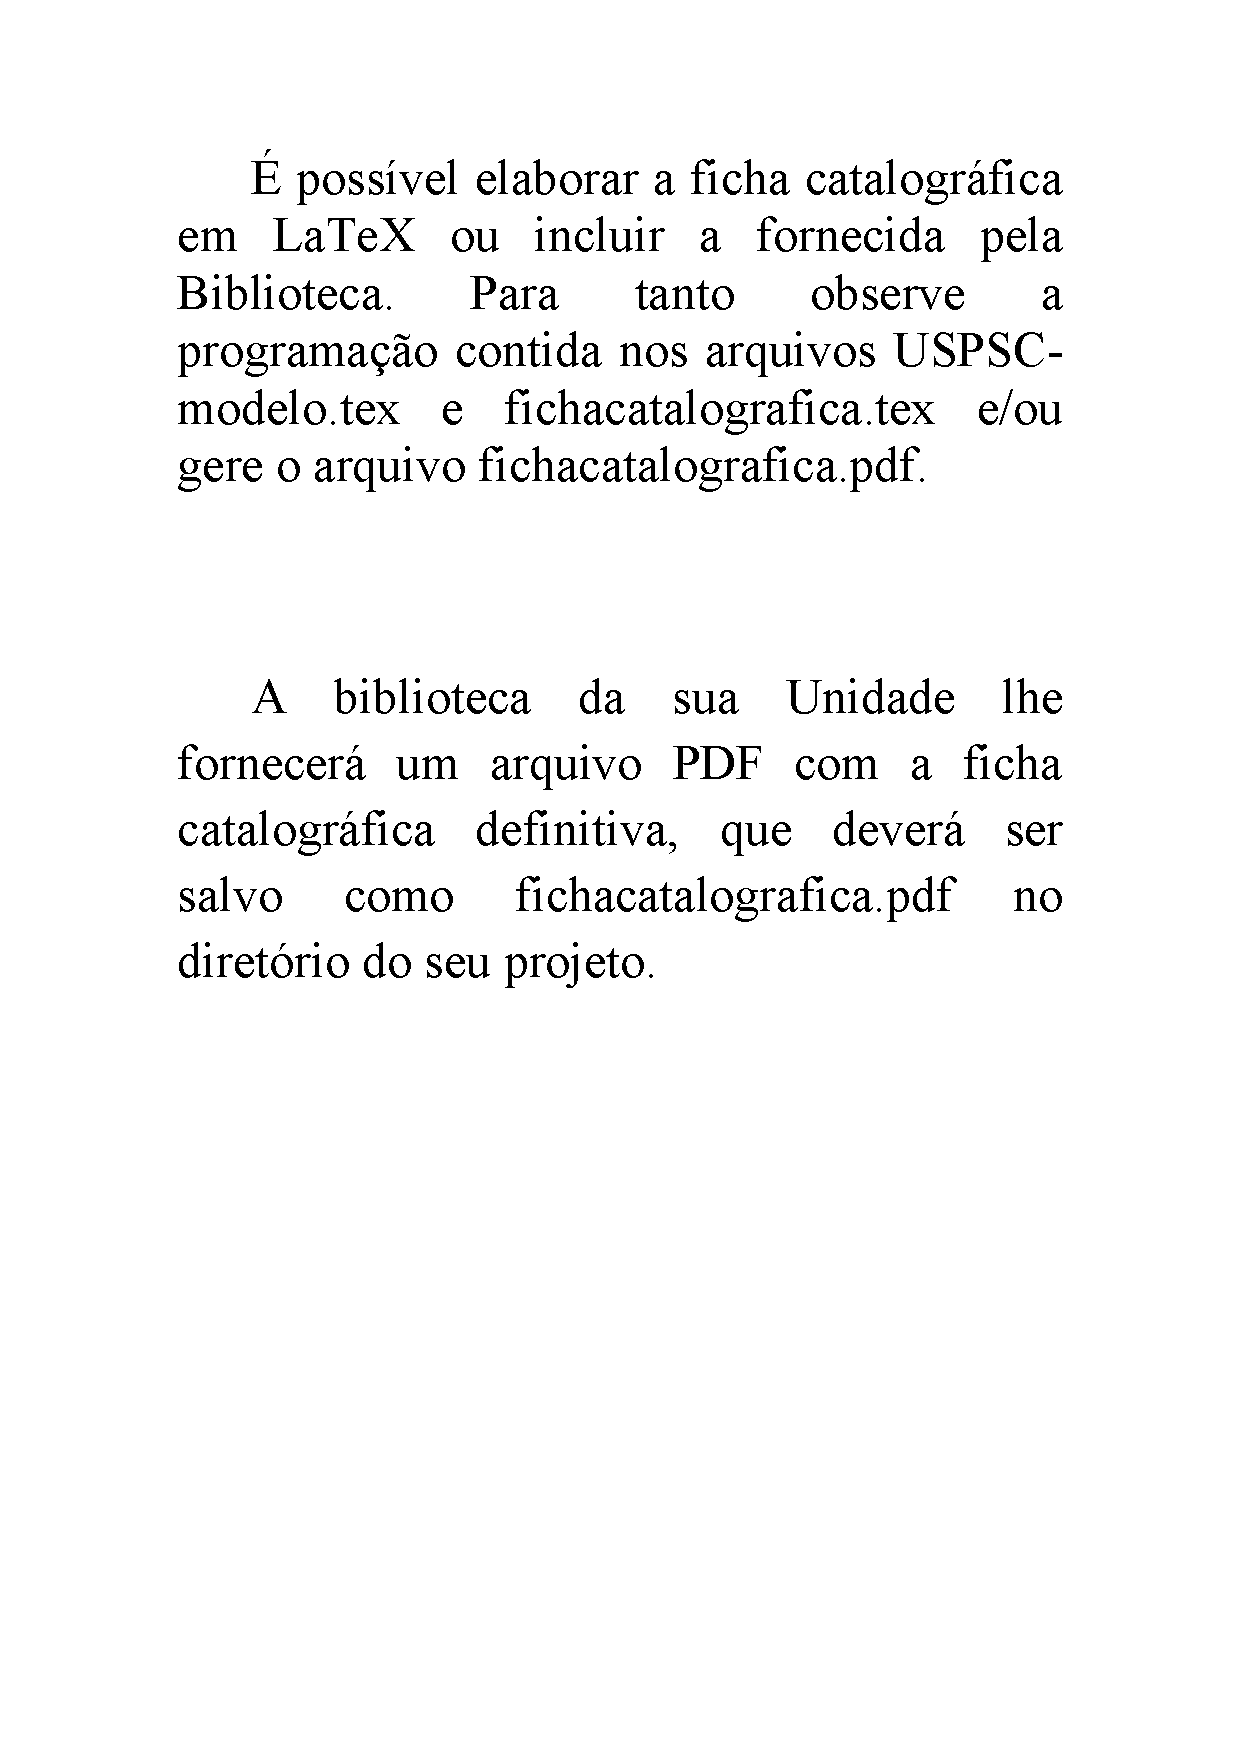
\includepdf{fichacatalografica.pdf}
			 %\end{fichacatalografica}
			 % Se você optar por elaborar a ficha catalográfica, deverá 
			 % incluir uma % antes das 3 linhas acima e tirar a % antes
			 % do comando % ---
% Inserir a ficha bibliografica
% ---
% Isto é um exemplo de Ficha Catalográfica, ou ``Dados internacionais de
% catalogação-na-publicação''. Você pode utilizar este modelo como referência. 
% Porém, provavelmente a biblioteca da sua universidade lhe fornecerá um PDF
% com a ficha catalográfica definitiva após a defesa do trabalho. Quando estiver
% com o documento, salve-o como PDF no diretório do seu projeto e substitua todo
% o conteúdo de implementação deste arquivo pelo comando abaixo:
%
\begin{fichacatalografica}
	\hspace{-1.4cm}
	\imprimirnotaautorizacao \\ \\
	%\sffamily
	\vspace*{\fill}					% Posição vertical
	\begin{center}					% Minipage Centralizado
		\imprimirnotabib \\
\begin{table}[htb]
	\scriptsize
	\centering	
	\begin{tabular}{|p{0.9cm} p{8.7cm}|}
		\hline
	      & \\
		  &	  \imprimirautorficha     \\
		
		 \imprimircutter & 
							\hspace{0.4cm}\imprimirtitulo~  / ~\imprimirautor~ ;  ~\imprimirorientadorcorpoficha. -- 	\imprimirlocal, \imprimirdata.   \\
		
		  &  % Para incluir nota referente à versão corrigida no corpo da ficha,
			  % incluir % no início da linha acima e tirar a % do início da linha abaixo
			  %	\hspace{0.4cm} \imprimirtitulo~  / ~\imprimirautor~ ; ~\imprimirorientadorcorpoficha~- ~\imprimirnotafolharosto. -- \imprimirlocal, \imprimirdata.  \\
		
			\hspace{0.4cm}\pageref{LastPage} p. : il. (algumas color.) ; 30 cm.\\ 
		  & \\
		  & 
		    \hspace{0.4cm}\imprimirnotaficha ~--~ 
						  \imprimirunidademin, 
						  \imprimiruniversidademin, 
		                  \imprimirdata. \\ 
		  & \\                 
		   % Para incluir nota referente à versão corrigida em notas,
		    % incluir uma % no início da linha acima e	
		    % tirar a % do início da linha abaixo
		    % & \hspace{0.4cm}\imprimirnotafolharosto \\ 
		  & \\ 
		  & \hspace{0.4cm}1. LaTeX. 2. abnTeX. 3. Classe USPSC. 4. Editoração de texto. 5. Normalização da documentação. 6. Tese. 7. Dissertação. 8. Documentos (elaboração). 9. Documentos eletrônicos. I. \imprimirorientadorficha. 
		   II. Título. \\
	
		     %Se houver co-orientador, inclua % antes da linha (antes de II. Título.) 
		     %          e tire a % antes do comando abaixo 
		     %III. Título. \\   
		  \hline
	\end{tabular}
\end{table}
	\end{center}
\end{fichacatalografica}
% ---


			 % ---
% Inserir a ficha bibliografica
% ---
% Isto é um exemplo de Ficha Catalográfica, ou ``Dados internacionais de
% catalogação-na-publicação''. Você pode utilizar este modelo como referência. 
% Porém, provavelmente a biblioteca da sua universidade lhe fornecerá um PDF
% com a ficha catalográfica definitiva após a defesa do trabalho. Quando estiver
% com o documento, salve-o como PDF no diretório do seu projeto e substitua todo
% o conteúdo de implementação deste arquivo pelo comando abaixo:
%
\begin{fichacatalografica}
	\hspace{-1.4cm}
	\imprimirnotaautorizacao \\ \\
	%\sffamily
	\vspace*{\fill}					% Posição vertical
	\begin{center}					% Minipage Centralizado
		\imprimirnotabib \\
\begin{table}[htb]
	\scriptsize
	\centering	
	\begin{tabular}{|p{0.9cm} p{8.7cm}|}
		\hline
	      & \\
		  &	  \imprimirautorficha     \\
		
		 \imprimircutter & 
							\hspace{0.4cm}\imprimirtitulo~  / ~\imprimirautor~ ;  ~\imprimirorientadorcorpoficha. -- 	\imprimirlocal, \imprimirdata.   \\
		
		  &  % Para incluir nota referente à versão corrigida no corpo da ficha,
			  % incluir % no início da linha acima e tirar a % do início da linha abaixo
			  %	\hspace{0.4cm} \imprimirtitulo~  / ~\imprimirautor~ ; ~\imprimirorientadorcorpoficha~- ~\imprimirnotafolharosto. -- \imprimirlocal, \imprimirdata.  \\
		
			\hspace{0.4cm}\pageref{LastPage} p. : il. (algumas color.) ; 30 cm.\\ 
		  & \\
		  & 
		    \hspace{0.4cm}\imprimirnotaficha ~--~ 
						  \imprimirunidademin, 
						  \imprimiruniversidademin, 
		                  \imprimirdata. \\ 
		  & \\                 
		   % Para incluir nota referente à versão corrigida em notas,
		    % incluir uma % no início da linha acima e	
		    % tirar a % do início da linha abaixo
		    % & \hspace{0.4cm}\imprimirnotafolharosto \\ 
		  & \\ 
		  & \hspace{0.4cm}1. LaTeX. 2. abnTeX. 3. Classe USPSC. 4. Editoração de texto. 5. Normalização da documentação. 6. Tese. 7. Dissertação. 8. Documentos (elaboração). 9. Documentos eletrônicos. I. \imprimirorientadorficha. 
		   II. Título. \\
	
		     %Se houver co-orientador, inclua % antes da linha (antes de II. Título.) 
		     %          e tire a % antes do comando abaixo 
		     %III. Título. \\   
		  \hline
	\end{tabular}
\end{table}
	\end{center}
\end{fichacatalografica}
% ---


			 % As informações que compõem a ficha catalográfica estão 
			 % definidos no arquivo USPSC-pre-textual-UUUU.tex
			 % ---
			 \end{verbatim} 
			 				
É possível incluir ou não o Código Cutter na ficha catalográfica, conforme a seguinte orientação nos respectivos arquivos pré-textuais:

\begin{verbatim}
\cutter{S856m}
% Para gerar a ficha catalográfica sem o Código Cutter, basta 
% incluir uma % na linha acima e tirar a % da linha abaixo
%\cutter{ } 
\end{verbatim} 

Através do arquivo fichacatalografica.tex é possível elaborar a ficha catalográfica em \LaTeX\ . Caso o trabalho possua co-orientador será necessário seguir as orientações contidas também no arquivo com os elementos pré-textuais.	 


\section{Resultados de comandos}\label{sec-divisoes}

O conteúdo desta seção foi baseado no item \textbf{1 Resultados de comandos} do \textbf{Modelo canônico de trabalho acadêmico com abnTEX2} \cite{equipeabntex2}.

% ---
\subsection{Codificação dos arquivos: UTF8}
% ---

A codificação \texttt{UTF8} deve ser utilizada para todos os arquivos do \abnTeX\ . Utilize a mesma codificação nos documentos que escrever, incluindo nos arquivos de base bibliográficas |.bib|. Para tanto, tanto o arquivo USPSC-modelo.tex  quanto o USPSC-TCC-modelo.tex devem conter o seguinte pacote:

\begin{verbatim}
\usepackage[utf8]{inputenc}	 % Codificacao do documento (conversão
                               automática dos acentos)
\end{verbatim}

% ---
\subsection{Diferentes idiomas e hifenizações}
\label{sec-hifenizacao}
% ---

Para usar hifenizações de diferentes idiomas, inclua nas opções do documento o
nome dos idiomas que o seu texto contém. Os usuários da Classe USPSC devem utilizar:

\begin{verbatim}
\documentclass[
% -- opções da classe memoir --
12pt,		% tamanho da fonte
openright,	% capítulos começam em pág ímpar (insere página vazia caso 
preciso)
twoside,  % para impressão em anverso (frente) e verso. Oposto a oneside - 
Nota: utilizar \imprimirfolhaderosto*
%oneside, % para impressão em páginas separadas (somente anverso) -  
Nota: utilizar \imprimirfolhaderosto
% inclua uma % antes do comando twoside e exclua a % antes do oneside 
a4paper,			% tamanho do papel. 
% -- opções da classe abntex2 --
chapter=TITLE,		% títulos de capítulos convertidos em letras 
maiúsculas
% -- opções do pacote babel --
english,			% idioma adicional para hifenização
french,				% idioma adicional para hifenização
spanish,			% idioma adicional para hifenização
brazil				% o último idioma é o principal do documento
% {uspsc} configura o cabeçalho contendo apenas o número da página
]{uspsc}
%]{uspsc1}
% Inclua % antes de ]{uspsc} e retire a % antes de %]{uspsc1}
% para utilizar o cabeçalho diferenciado para as páginas pares e ímpares 
como indicado abaixo:
%- páginas ímpares: cabeçalho com seções ou subseções e o número da página
%- páginas pares: cabeçalho com o número da página e o título do capítulo 
% ---
\end{verbatim}

Desta forma o texto deverá ser escrito idioma português-brasileiro (\texttt{brazil}), podendo ter citações em inglês, francês e espanhol.

O idioma português-brasileiro (\texttt{brazil}) é incluído automaticamente pela
classe \textsf{abntex2}. Porém, mesmo assim a opção \texttt{brazil} deve ser
informada como a última opção da classe para que todos os pacotes reconheçam o
idioma. Vale ressaltar que a última opção de idioma é a utilizada por padrão no
documento. 

Portanto, para Classe USPSC, caso deseje escrever um texto em inglês que tenha
citações em espanhol, português e francês, você deverá usar:

\begin{verbatim}
\documentclass[
% -- opções da classe memoir --
12pt,		% tamanho da fonte
openright,	% capítulos começam em pág ímpar (insere página vazia caso 
preciso)
twoside,  % para impressão em anverso (frente) e verso. Oposto a oneside - 
Nota: utilizar \imprimirfolhaderosto*
%oneside, % para impressão em páginas separadas (somente anverso) -  
Nota: utilizar \imprimirfolhaderosto
% inclua uma % antes do comando twoside e exclua a % antes do oneside 
a4paper,			% tamanho do papel. 
% -- opções da classe abntex2 --
chapter=TITLE,		% títulos de capítulos convertidos em letras 
maiúsculas
% -- opções do pacote babel --
spanish,			% idioma adicional para hifenização
french,				% idioma adicional para hifenização
brazil,				% o último idioma é o principal do documento
english 			% idioma adicional para hifenização
% {uspsc} configura o cabeçalho contendo apenas o número da página
]{uspsc}
%]{uspsc1}
% Inclua % antes de ]{uspsc} e retire a % antes de %]{uspsc1}
% para utilizar o cabeçalho diferenciado para as páginas pares e ímpares 
como indicado abaixo:
%- páginas ímpares: cabeçalho com seções ou subseções e o número da página
%- páginas pares: cabeçalho com o número da página e o título do capítulo 
% ---
\end{verbatim}

A lista completa de idiomas suportados, bem como outras opções de hifenização,
estão disponíveis em \citeonline[p.~7-8]{babel2011}.

Exemplo de hifenização em inglês\footnote{Extraído de:
	\url{http://en.wikibooks.org/wiki/LaTeX/Internationalization}}:

\begin{otherlanguage*}{english}
	\textit{Text in English language. This environment switches all language-related
		definitions, like the language specific names for figures, tables etc. to the other
		language. The starred version of this environment typesets the main text
		according to the rules of the other language, but keeps the language specific
		string for ancillary things like figures, in the main language of the document.
		The environment hyphenrules switches only the hyphenation patterns used; it can
		also be used to disallow hyphenation by using the language name
		`nohyphenation'.}
\end{otherlanguage*}

Exemplo de hifenização em francês\footnote{Extraído de:
	\url{http://bigbrowser.blog.lemonde.fr/2013/02/17/tu-ne-tweeteras-point-le-vatican-interdit-aux-cardinaux-de-tweeter-pendant-le-conclave/}}:

\begin{otherlanguage*}{french}
	\textit{Texte en français. Pas question que Twitter ne vienne faire une
		concurrence déloyale à la traditionnelle fumée blanche qui marque l'élection
		d'un nouveau pape. Pour éviter toute fuite précoce, le Vatican a donc pris un
		peu d'avance, et a déjà interdit aux cardinaux qui prendront part au vote
		d'utiliser le réseau social, selon Catholic News Service. Une mesure valable
		surtout pour les neuf cardinaux – sur les 117 du conclave – pratiquants très
		actifs de Twitter, qui auront interdiction pendant toute la période de se
		connecter à leur compte.}
\end{otherlanguage*}

Exemplo de hifenização em espanhol\footnote{Extraído de:
	\url{http://internacional.elpais.com/internacional/2013/02/17/actualidad/1361102009_913423.html}}:

\foreignlanguage{spanish}{\textit{Decenas de miles de personas ovacionan al pontífice en su
		penúltimo ángelus dominical, el primero desde que anunciase su renuncia. El Papa se
		centra en la crítica al materialismo}}.

O idioma geral do texto pode ser alterado como no exemplo seguinte:

\begin{verbatim}
\selectlanguage{english}

\end{verbatim}

Isso altera automaticamente a hifenização e todos os nomes constantes de
referências do documento para o idioma inglês. Consulte o manual da classe para obter orientações adicionais sobre internacionalização de documentos produzidos com \textsf{\abnTeX} \cite{abnetxclasse}.

% ---
\subsection{Enumerações}
% ---

\index{alíneas}\index{subalíneas}\index{incisos}Quando for necessário enumerar
os diversos assuntos de uma seção que não possua título, esta deve ser
subdividida em alíneas \cite[4.2]{nbr6024}:

\begin{alineas}

  \item os diversos assuntos que não possuam título próprio, dentro de uma mesma
  seção, devem ser subdivididos em alíneas; 
  
  \item o texto que antecede as alíneas termina em dois pontos;
  \item as alíneas devem ser indicadas alfabeticamente, em letra minúscula
  seguida de parêntese. Utilizam-se letras dobradas, quando esgotadas as
  letras do alfabeto;

  \item as letras indicativas das alíneas devem apresentar recuo em relação à
  margem esquerda;

  \item o texto da alínea deve começar por letra minúscula e terminar em
  ponto-e-vírgula, exceto a última alínea que termina em ponto final;

  \item o texto da alínea deve terminar em dois pontos, se houver subalínea;

  \item a segunda e as seguintes linhas do texto da alínea começa sob a
  primeira letra do texto da própria alínea;
  
  \item subalíneas \cite{nbr6024} devem ser conforme as alíneas a
  seguir:

  \begin{alineas}
     \item as subalíneas devem começar por travessão seguido de espaço;

     \item as subalíneas devem apresentar recuo em relação à alínea;

     \item o texto da subalínea deve começar por letra minúscula e terminar em
     ponto-e-vírgula. A última subalínea deve terminar em ponto final, se não
     houver alínea subsequente;

     \item a segunda e as seguintes linhas do texto da subalínea começam sob a
     primeira letra do texto da própria subalínea.
  \end{alineas}
  
  \item no \abnTeX\ estão disponíveis os ambientes \texttt{incisos} e
  \texttt{subalineas}, que em suma é o mesmo que se criar outro nível de
  \texttt{alineas}, como nos exemplos à seguir:
  
  \begin{incisos}
    \item \textit{Um novo inciso em itálico};
  \end{incisos}
  
  \item Alínea em \textbf{negrito}:
  
  \begin{subalineas}
    \item \textit{Uma subalínea em itálico};
    \item \underline{\textit{Uma subalínea em itálico e sublinhado}}; 
  \end{subalineas}
  
  \item Última alínea com \emph{ênfase}.
  
\end{alineas}

% ---
\subsection{Espaçamento entre parágrafos e linhas}\label{sec_espacamento}
% ---

\index{espaçamento!dos parágrafos}O tamanho do parágrafo, espaço entre a margem
e o início da frase do parágrafo, é definido por:

\begin{verbatim}
   \setlength{\parindent}{1.3cm}
\end{verbatim}

\index{espaçamento!do primeiro parágrafo}Por padrão, não há espaçamento no
primeiro parágrafo de cada início de divisão do documento
(\autoref{sec-divisoes-b}). Porém, você pode definir que o primeiro parágrafo
também seja indentado, como é o caso deste documento. Para isso, apenas inclua o
pacote \textsf{indentfirst} no preâmbulo do documento:

\begin{verbatim}
   \usepackage{indentfirst} % Indenta o primeiro parágrafo de cada seção.
\end{verbatim}

\index{espaçamento!entre os parágrafos}O espaçamento entre um parágrafo e outro
pode ser controlado por meio do comando:

\begin{verbatim}
  \setlength{\parskip}{0.2cm}  % tente também \onelineskip
\end{verbatim}

\index{espaçamento!entre as linhas}O controle do espaçamento entre linhas é
definido por:
\begin{verbatim}
  \OnehalfSpacing       % espaçamento um e meio (padrão); 
  \DoubleSpacing        % espaçamento duplo
  \SingleSpacing        % espaçamento simples	
\end{verbatim}

Para isso, também estão disponíveis os ambientes:
\begin{verbatim}
  \begin{SingleSpace} ...\end{SingleSpace}
  \begin{Spacing}{hfactori} ... \end{Spacing}
  \begin{OnehalfSpace} ... \end{OnehalfSpace}
  \begin{OnehalfSpace*} ... \end{OnehalfSpace*}
  \begin{DoubleSpace} ... \end{DoubleSpace}
  \begin{DoubleSpace*} ... \end{DoubleSpace*} 
\end{verbatim}

% ---
\subsection{Tabelas}

As tabelas e os quadros apresentam os dados de modo resumido, oferecendo uma visão geral do conteúdo em questão, visando facilitar a compreensão do fenômeno em estudo. A diferença básica entre ambas está relacionada ao conteúdo e a formatação. 

Tabela é o conjunto de dados estatísticos, dispostos em determinada ordem de classificação, que expressam as variações qualitativas de um fenômeno. Sua finalidade básica é resumir ou sintetizar dados \cite{sibi2009}.

A construção de tabelas deve obedecer os critérios estabelecidos pelo Instituto Brasileiro de Geografia e Estatística (IBGE) e requerido pelas normas da ABNT para documentos técnicos e acadêmicos.

A \autoref{tab-ibge} é um exemplo de tabela alinhada que pode ser longa ou curta, conforme padrão do IBGE.

\begin{table}[htb]
	%\begin{table}[H]
	\IBGEtab{%
		\caption{Frequência anual por categoria de usuários}%
		\label{tab-ibge}
	}{%
	\begin{tabular}{ccc}
		\toprule
		Categoria de Usuários & Frequência de Usuários \\
		\midrule \midrule
		Graduação & 72\% \\
		\midrule 
		Pós-Graduação & 15\% \\
		\midrule 
		Docente & 10\% \\
		\midrule 
		Outras & 3\% \\
		\bottomrule
	\end{tabular}%
}{%
\fonte{Elaborada pelos autores.}%
\nota{Exemplo de uma nota.}%
\nota[Anotações]{Uma anotação adicional, que pode ser seguida de várias
	outras.}%

}
\end{table}


\begin{table}[H]
	\IBGEtab{%
		\caption{Níveis descritivos dos testes de comparação de médias entre grupos para profundidade da lesão junto à restauração}%
		\label{tabela-ibge}
	}{%
	\begin{tabular}{p{5.5cm}|p{5.5cm}}
		\hline
		\textbf{Resultado} & \textbf{Nível Descritivo} \\ 
		\hline 
		CIC < Ariston & < 0,0001  \\
		Ariston < Am & 0,0118  \\
		Am = Helio & 0,4576  \\
		-100 = Helio & 0,3360  \\
		\hline
	\end{tabular}%
}{%
\fonte{\citeonline{sibi2009}}%
}
\end{table} 

Os \textbf{(APÊNDICES H-I)} exemplificam outras formatações de tabelas.
% ---
\subsection{Figuras}\label{sec_figuras}
% ---

\index{figuras}Figuras podem ser criadas diretamente em \LaTeX,
como o exemplo da \autoref{fig_circulo}. \\ 


\begin{figure}[htb]
	\caption{\label{fig_circulo}A delimitação do espaço}
	\begin{center}
		\setlength{\unitlength}{9cm}
		\begin{picture}(1,1)
		\put(0,0){\line(0,1){1}}
		\put(0,0){\line(1,0){1}}
		\put(0,0){\line(1,1){1}}
		\put(0,0){\line(1,2){.5}}
		\put(0,0){\line(1,3){.3333}}
		\put(0,0){\line(1,4){.25}}
		\put(0,0){\line(1,5){.2}}
		\put(0,0){\line(1,6){.1667}}
		\put(0,0){\line(2,1){1}}
		\put(0,0){\line(2,3){.6667}}
		\put(0,0){\line(2,5){.4}}
		\put(0,0){\line(3,1){1}}
		\put(0,0){\line(3,2){1}}
		\put(0,0){\line(3,4){.75}}
		\put(0,0){\line(3,5){.6}}
		\put(0,0){\line(4,1){1}}
		\put(0,0){\line(4,3){1}}
		\put(0,0){\line(4,5){.8}}
		\put(0,0){\line(5,1){1}}
		\put(0,0){\line(5,2){1}}
		\put(0,0){\line(5,3){1}}
		\put(0,0){\line(5,4){1}}
		\put(0,0){\line(5,6){.8333}}
		\put(0,0){\line(6,1){1}}
		\put(0,0){\line(6,5){1}}
		\end{picture}
	\end{center}
	\legend{Fonte: \citeonline{equipeabntex2}}
\end{figure}

Outra opção é incorporar a figura utilizando um arquivo externo, como é o caso da \autoref{fig_grafico}. Se a figura que for incluída se tratar de um diagrama, um gráfico ou uma ilustração, que você mesmo produza, priorize o uso de imagens vetoriais no formato PDF. Com isso, o tamanho do arquivo final do trabalho será menor e as imagens terão uma apresentação melhor, principalmente quando impressas, uma vez que imagens vetoriais são perfeitamente escaláveis para qualquer dimensão. Nesse caso, se for utilizar o Microsoft Excel para produzir gráficos, ou o Microsoft Word para ilustrações, exporte-os como PDF e os incorpore ao documento conforme o exemplo abaixo. No entanto, para manter a
coerência no uso de software livre (já que você está usando \LaTeX\  e \abnTeX),
teste a ferramenta \textsf{InkScape}\index{InkScape}
(\url{http://inkscape.org/}). Ela é uma excelente opção de código-livre para
produzir ilustrações vetoriais, similar ao CorelDraw\index{CorelDraw} ou ao Adobe
Illustrator\index{Adobe Illustrator}. De todo modo, caso não seja possível
utilizar arquivos de imagens como PDF, utilize qualquer outro formato, como
JPEG, GIF, BMP, etc. Nesse caso, você pode tentar aprimorar as imagens
incorporadas com o software livre \textsf{Gimp}\index{Gimp}
(\url{http://www.gimp.org/}). Ele é uma alternativa livre ao Adobe
Photoshop\index{Adobe Photoshop}. \\

\begin{figure}[H]
	\caption{\label{fig_grafico}Gráfico produzido em Excel e salvo como PDF}
	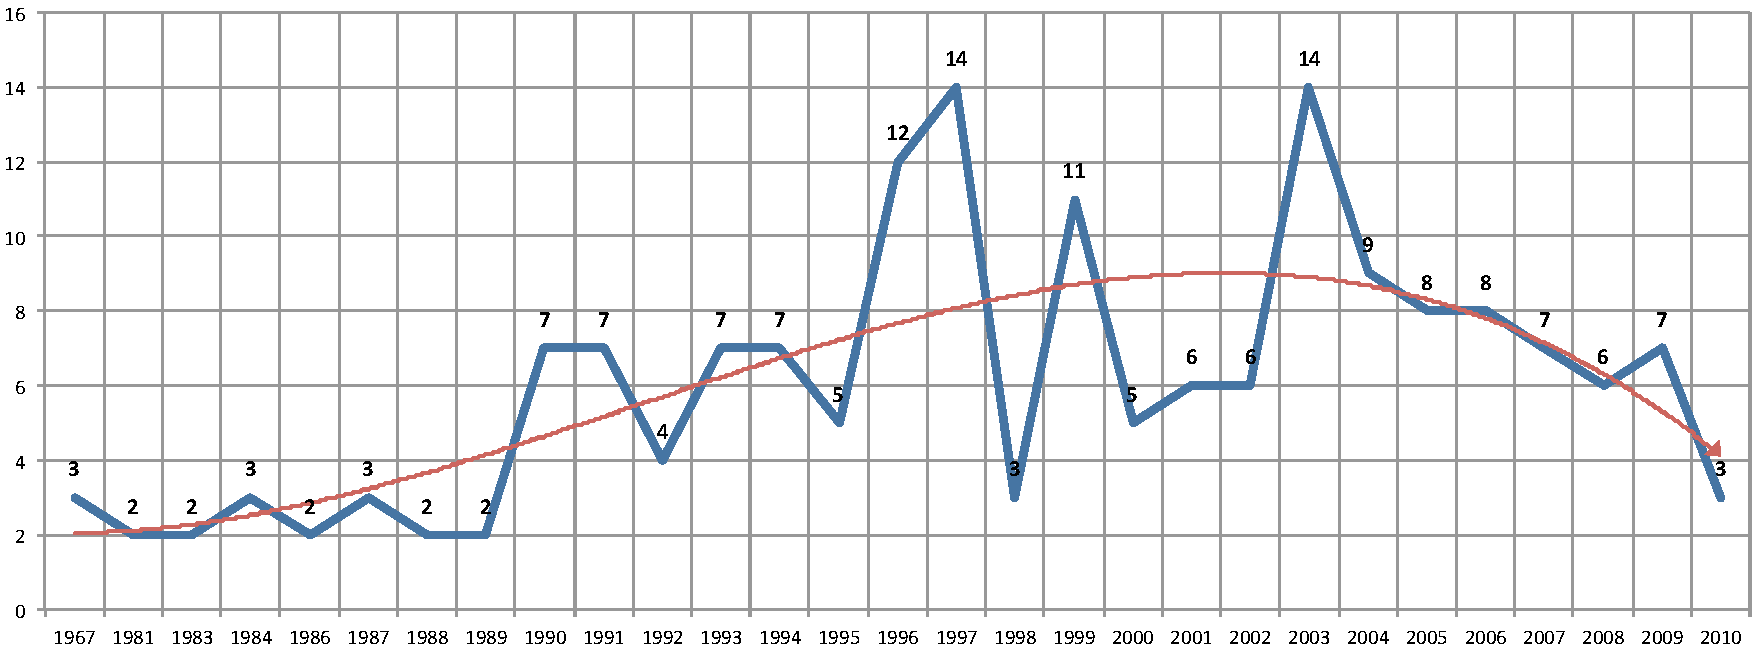
\includegraphics[scale=0.5]{USPSC-modelo-img-grafico.pdf}
	\begin{flushleft}
		Fonte: \citeonline[p. 24]{araujo2012}
	\end{flushleft}	
\end{figure}


A formatação do quadro é similar à tabela, mas deve ter suas laterais fechadas e conter as linhas horizontais.

% o comando \newpage foi utilizado para forçar a quebra de página

\begin{quadro}[htb]
	\caption{\label{quadro_modelo}Níveis de investigação}
	\begin{tabular}{|p{2.6cm}|p{6.0cm}|p{2.25cm}|p{3.40cm}|}
		\hline
		\textbf{Nível de Investigação} & \textbf{Insumos}  & \textbf{Sistemas de Investigação}  & \textbf{Produtos}  \\
		\hline
		Meta-nível & Filosofia\index{filosofia} da Ciência  & Epistemologia &
		Paradigma  \\
		\hline
		Nível do objeto & Paradigmas do metanível e evidências do nível inferior &
		Ciência  & Teorias e modelos \\
		\hline
		Nível inferior & Modelos e métodos do nível do objeto e problemas do nível inferior & Prática & Solução de problemas  \\
		\hline
	\end{tabular}
	\begin{flushleft}
		%\fonte{\citeonline{van1986}}
		Fonte: \citeonline{van1986}
	\end{flushleft}
\end{quadro} 


Os \textbf{(APÊNDICES B-F)} são exemplos de quadros.

% ---
\subsubsection{Figuras em minipages}
% ---

As ilustrações devem sempre ter numeração contínua e única em todo o documento:

% O comando \newpage força a quebra de página

\begin{citacao}
	Qualquer que seja o tipo de ilustração, sua identificação aparece na parte
	superior, precedida da palavra designativa (desenho, esquema, fluxograma,
	fotografia, gráfico, mapa, organograma, planta, quadro, retrato, figura,
	imagem, entre outros), seguida de seu número de ordem de ocorrência no texto,
	em algarismos arábicos, travessão e do respectivo título. Após a ilustração, na
	parte inferior, indicar a fonte consultada (elemento obrigatório, mesmo que
	seja produção do próprio autor), legenda, notas e outras informações
	necessárias à sua compreensão (se houver). A ilustração deve ser citada no
	texto e inserida o mais próximo possível do trecho a que se
	refere \cite{nbr14724}.
\end{citacao}

\emph{Minipages} são usadas para inserir textos ou outros elementos em quadros
com tamanhos e posições controladas. Veja o exemplo da
\autoref{fig_minipage_imagem1} e da \autoref{fig_minipage_grafico2}.

\begin{figure}[H]
	\label{teste}
	\centering
	\begin{minipage}{0.4\textwidth}
		\centering
		\caption{Imagem 1 da minipage} \label{fig_minipage_imagem1}
		
\includegraphics[scale=0.9]{USPSC-modelo-img-marca.pdf}
		\legend{Fonte: \citeonline{equipeabntex2}}
	\end{minipage}
	\hfill
	\begin{minipage}{0.4\textwidth}
		\centering
		\caption{Grafico 2 da minipage} \label{fig_minipage_grafico2}
		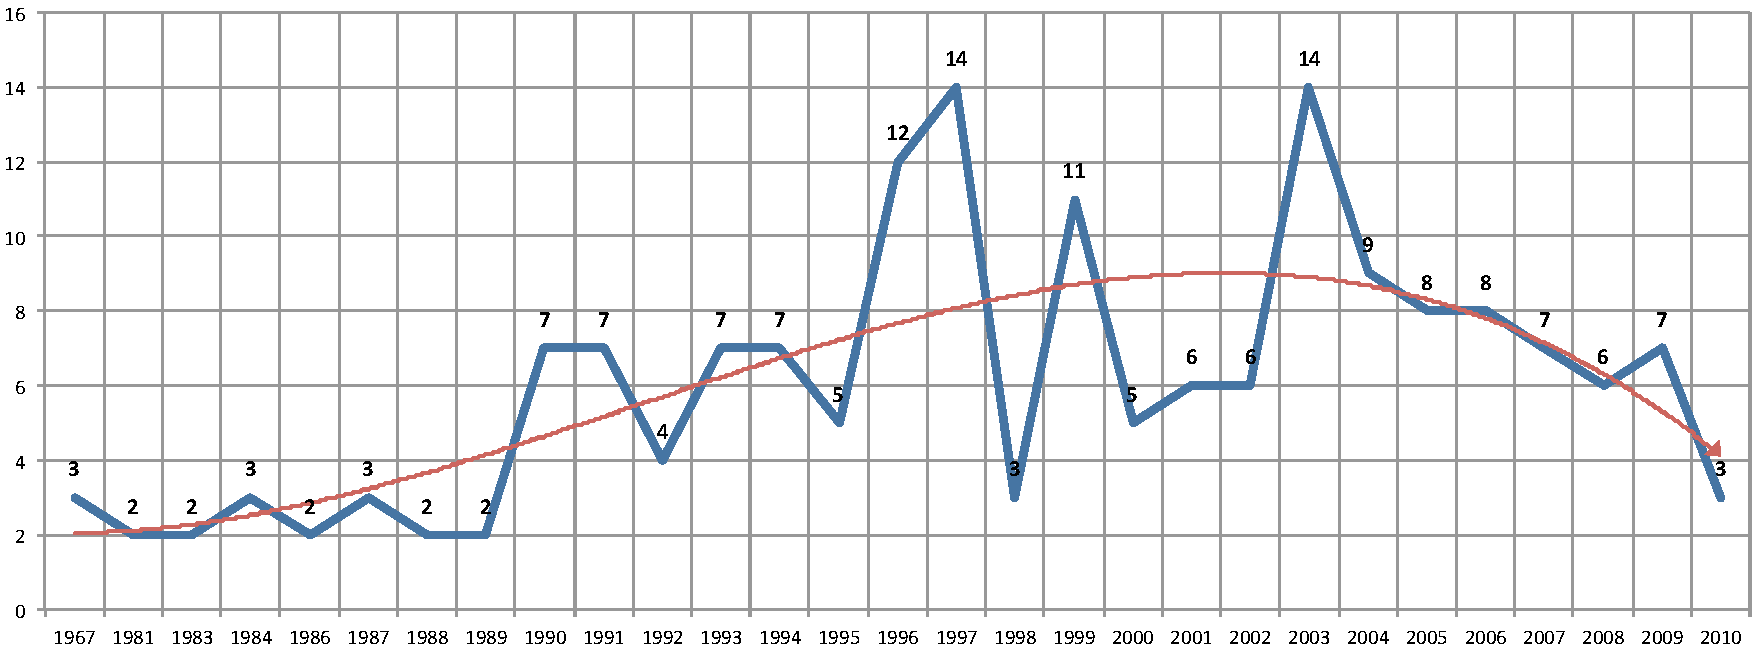
\includegraphics[scale=0.2]{USPSC-modelo-img-grafico.pdf}
		\legend{Fonte: \citeonline[p. 24]{araujo2012}}
	\end{minipage}
\end{figure}

% ---
\subsection{Expressões matemáticas}
% ---

\index{expressões matemáticas}Use o ambiente \texttt{equation} para escrever
expressões matemáticas numeradas:

\begin{equation}
\forall x \in X, \quad \exists \: y \leq \epsilon
\end{equation}

Escreva expressões matemáticas entre \$ e \$, como em $ \lim_{x \to \infty}
\exp(-x) = 0 $, para que fiquem na mesma linha.

Também é possível usar colchetes para indicar o início de uma expressão
matemática que não é numerada.

\[
\left|\sum_{i=1}^n a_ib_i\right|
\le
\left(\sum_{i=1}^n a_i^2\right)^{1/2}
\left(\sum_{i=1}^n b_i^2\right)^{1/2}
\]

Consulte mais informações sobre expressões matemáticas em
\url{https://github.com/abntex/abntex2/wiki/Referencias}.


% ---
\subsection{Estruturas, reações e mecanismos de reações químicas}
% ---
O pacote chemfig permite o desenho de estruturas, reações e mecanismos de reações químicas em latex. Abaixo relacionamos alguns exemplos de utilização de seus recursos e indicamos a consulta do Chemfig Manual para mais informações.

A fórmula estrutural do metano é:
\begin{center}
	\chemfig{C(-[5]H)(-[2]H)(<[:-70]H)(<:[:-20]H)}
	
\end{center}


A fórmula estrutural do 1-hexeno é:
\begin{center}
	\chemfig{H_3C-[,1.5]{{(CH_2)}_3}-[,1.5]CH=CH_2}
	
\end{center}



Molecula da Adrenalina
\begin{center}
\chemfig{*6((-HO)-=-(-(<[::60]OH)-[::-60]-[::-60,,,2]
	HN-[::+60]CH_3)=-(-HO)=)}


\end{center}



Exemplo de reações químicas:

\begin{center}
	\schemestart
	\chemfig{-[:30](-[2])-[:-30]OH}
	\arrow
	\chemfig{-[:30](-[2])=^[:-30]O}
	\schemestop
	
\end{center}

Mais um exemplo de reações químicas:
\begin{center}\small\setatomsep{1.5em}
	\schemestart
	\chemfig{*6(=-=(-(=[2]O)-[::-60]O-[0]O-[::30](=[2]O)-[::-60]*6(=-=-=-))-=-)}
	\arrow{->[$\Delta$]}
	2 \chemfig{*6(=-=(-(=[2]O)-[::-60]\lewis{0.,O})-=-)}
	\arrow
	2 \chemfig{*6(=-=(-[,.15,,,draw=none]\lewis{0.,})-=-)}\+\ch{2 CO2 ^}
	\schemestop
	
	
\end{center}

Os exemplos abaixo ilustram que é possível modificar cores, utilizar o recurso de perspectiva, dentre outros recursos que obter destaques.


Mudando as cores das moleculas
\begin{center}
\chemfig{C|{\color{blue}H_3}-C(=[1]O)-[7]O|{\color{red}H}}


\end{center}


Moleculas em perspectiva
\begin{center}
	\setcrambond{2pt}{}{}
	\chemfig{HO-[2,0.5,2]?<[7,0.7]-[,,,,
		line width=2pt]>[1,0.7]-[3,0.7]O-[4]?}
	
	
\end{center}


% ---
\subsection{Inclusão de outros arquivos}\label{sec-include}
% ---

É uma boa prática dividir o seu documento em diversos arquivos, e não
apenas escrever tudo em um único. Esse recurso foi utilizado neste
documento. Para incluir diferentes arquivos em um arquivo principal,
de modo que cada arquivo incluído fique em uma página diferente, utilize o
comando:

\begin{verbatim}
   \include{documento-a-ser-incluido}      % sem a extensão .tex
\end{verbatim}

Para incluir documentos sem quebra de páginas, utilize:

\begin{verbatim}
   \input{documento-a-ser-incluido}      % sem a extensão .tex
\end{verbatim}
% ---
\subsection{Índice(s)}
% ---
Elemento opcional, que consiste em lista de palavras ou frases ordenadas alfabeticamente (autor, título ou assunto) ou sistematicamente (ordenação por classes, numérica ou cronológica); localiza e remete para as informações contidas no texto. A paginação deve ser contínua, dando seguimento ao texto principal \cite{sibi2009}.

Para criar índice remissivo no \LaTeX\  utilize o pacote makeidx, que deve estar declarado com os demais pacotes. No presente modelo está declarado no arquivo USPSC-modelo.tex, conforme indicado abaixo:

\begin{verbatim}
% ---
% Pacotes básicos - Fundamentais 
% ---
\usepackage[T1]{fontenc}		% Selecao de codigos de fonte.
\usepackage[utf8]{inputenc}		% Codificacao do documento (conversão 
automática dos acentos)
\usepackage{lmodern}			% Usa a fonte Latin Modern
% Para utilizar a fonte Times New Roman, inclua uma % no início do comando 
acima  "\usepackage{lmodern}"
% Lembre-se de alterar a fonte no comando que imprime o preâmbulo no 
arquivo da Classe USPSC.cls
%\usepackage{times}			% Usa a fonte Times New Roman					
\usepackage{lastpage}			% Usado pela Ficha catalográfica
\usepackage{indentfirst}		% Indenta o primeiro parágrafo de cada seção.
\usepackage{color}				% Controle das cores
\usepackage{graphicx}			% Inclusão de gráficos
\usepackage{float} 				%Fixa tabelas e figuras no local exato
\usepackage{microtype} 			% para melhorias de justificação
\usepackage{pdfpages}
\usepackage[labelsep=endash]{caption}
\usepackage{makeidx}            % para gerar índice remissimo
% ---
\end{verbatim}

A habilitação dos comandos de indexação foi incluída no arquivo USPSC-modelo.tex da seguinte forma:


\begin{verbatim}
% compila o sumário e índice
\makeindex
% ---
\end{verbatim}

O presente modelo inclui um exemplo de índice, gerado a partir da utilização de comandos similares aos reproduzidos abaixo:

\begin{verbatim}
\index{InkScape}
\index{CorelDraw}
\index{Adobe Illustrator}
\index{Gimp}
\index{Adobe Photoshop}
\index{espaçamento!do primeiro parágrafo}
\index{espaçamento!dos parágrafos}
\index{espaçamento!entre as linhas}
\index{espaçamento!entre os parágrafos}
\end{verbatim}

Os comandos acima estão no arquivo USPSC-Cap2-Desenvolvimento.tex, em textos na  \autoref{sec_figuras} e em \autoref{sec_espacamento}.

Para imprimir o índice, no final do arquivo USPSC-modelo.tex foi incluído:

\begin{verbatim}

%---------------------------------------------------------------------
% INDICE REMISSIVO
%--------------------------------------------------------------------
\phantompart
\printindex
%---------------------------------------------------------------------
\end{verbatim}

Para que o índice seja gerado e incluído corretamente no texto é necessário compilá-lo separadamente. No \textbf{TeXstudio 2.9.4}, na barra de menu, selecione \textbf{Tools} e execute \textbf{Index}.


% ---
\subsection{Compilar o documento \LaTeX}
% ---

Geralmente os editores \LaTeX, como o
TeXlipse\footnote{\url{http://texlipse.sourceforge.net/}}, o
Texmaker\footnote{\url{http://www.xm1math.net/texmaker/}}, entre outros,
compilam os documentos automaticamente, de modo que você não precisa se
preocupar com isso.

No entanto, você pode compilar os documentos \LaTeX\ usando os seguintes
comandos, que devem ser digitados no \emph{Prompt de Comandos} do Windows ou no
\emph{Terminal} do Mac ou do Linux:

\begin{verbatim}
   pdflatex ARQUIVO_PRINCIPAL.tex
   bibtex ARQUIVO_PRINCIPAL.aux
   makeindex ARQUIVO_PRINCIPAL.idx 
   makeindex ARQUIVO_PRINCIPAL.nlo -s nomencl.ist -o ARQUIVO_PRINCIPAL.nls
   pdflatex ARQUIVO_PRINCIPAL.tex
   pdflatex ARQUIVO_PRINCIPAL.tex
\end{verbatim}

% ---
\subsection{Remissões internas}
% ---

Ao nomear a \autoref{tab-ibge} e a \autoref{fig_circulo}, apresentamos um exemplo de remissão interna, que também pode ser feita quando indicamos o
\autoref{cap_exemplos}, que tem o nome \emph{\nameref{cap_exemplos}}. O número
do capítulo indicado é \ref{cap_exemplos}, que se inicia à
\autopageref{cap_exemplos}\footnote{O número da página de uma remissão pode ser
	obtida também assim:
	\pageref{cap_exemplos}.}.
Veja a \autoref{sec-divisoes-b} para outros exemplos de remissões internas entre
seções, subseções e subsubseções.

O código usado para produzir o texto desta seção é:

\begin{verbatim}
Ao nomear a \autoref{tab-nivinv} e a \autoref{fig_circulo}, apresentamos 
um exemplo de remissão interna, que também pode ser feita quando indicamos 
o \autoref{cap_exemplos}, que tem o nome \emph{\nameref{cap_exemplos}}. O
número do capítulo indicado é \ref{cap_exemplos}, que se inicia à 
\autopageref{cap_exemplos}\footnote{O número da página de uma remissão 
pode ser obtida também assim: \pageref{cap_exemplos}.}. Veja a 
\autoref{sec-divisoes-b} para outros exemplos de remissões internas entre 
seções, subseções e subsubseções.
\end{verbatim}

% ---
\section{Divisões do documento}\label{sec-divisoes-b}
Esta seção exemplifica o uso de divisões de documentos em conformidade com a ABNT NBR 6024  \cite{nbr6024}.
% ---
% ---
\subsection{Divisões do documento: subseção}\label{sec-divisoes-subsection}
% ---

Um exemplo de seção é a \autoref{sec-divisoes-b}. Esta é a \autoref{sec-divisoes-subsection}.

\subsubsection{Divisões do documento: subsubseção}\label{sec-divisoes-subsubsection}

Isto é uma \texttt{subsubsection} do \LaTeX, mas é denominada de ``subseção'' porque no português não temos a palavra ``subsubseção''.

\subsubsection{Divisões do documento: subsubseção}

Isto é outra subsubseção.

\subsection{Divisões do documento: subseção}\label{sec-exemplo-subsec}

Isto é uma subseção.

\subsubsection{Divisões do documento: subsubseção}

Isto é mais uma subsubseção da \autoref{sec-exemplo-subsec}.


\subsubsubsection{Esta é uma subseção de quinto
nível}\label{sec-exemplo-subsubsubsection}

Esta é uma seção de quinto nível. Ela é produzida com o seguinte comando:

\begin{verbatim}
\subsubsubsection{Esta é uma subseção de quinto
nível}\label{sec-exemplo-subsubsubsection}
\end{verbatim}

\subsubsubsection{Esta é outra subseção de quinto nível}\label{sec-exemplo-subsubsubsection-outro}

Esta é outra seção de quinto nível.


\paragraph{Este é um parágrafo numerado}\label{sec-exemplo-paragrafo}

Este é um exemplo de parágrafo nomeado. Ele é produzido com o comando de
parágrafo:

\begin{verbatim}
\paragraph{Este é um parágrafo nomeado}\label{sec-exemplo-paragrafo}
\end{verbatim}

A numeração entre parágrafos numerados e subsubsubseções são contínuas.

\paragraph{Esta é outro parágrafo numerado}\label{sec-exemplo-paragrafo-outro}

Este é outro parágrafo nomeado.

% ---
\subsection{Este é um exemplo de nome de subseção longa que se aplica a seções e demais divisões do documento. Ele deve estar alinhado à esquerda e a segunda e demais linhas devem iniciar logo abaixo da primeira palavra da primeira linha} 

Observe que o alinhamento do título obedece esta regra também no sumário.
	

% ---
\section{Manual da classe \textsf{\abnTeX}}
% ---

O manual da classe \textsf{\abnTeX} possui uma referência completa das macros e ambientes disponíveis \cite{abnetxclasse}.

Contém informações adicionais sobre as normas ABNT
observadas pelo \textsf{\abnTeX} e considerações sobre eventuais requisitos específicos
não atendidos, como o caso da ABNT NBR 14724 \cite{nbr14724}, que
especifica o espaçamento entre os capítulos e o início do texto, regra
propositalmente não atendida pelo presente modelo.

% ---
\section{Precisa de ajuda sobre \textsf{\abnTeX}?}
% ---

Consulte a FAQ com perguntas frequentes e comuns no portal do \textsf{\abnTeX}:
\url{https://github.com/abntex/abntex2/wiki/FAQ}.

Inscreva-se no grupo de usuários \LaTeX:
\url{http://groups.google.com/group/latex-br}, tire suas dúvidas e ajude
outros usuários.

Participe também do grupo de desenvolvedores do \textsf{\abnTeX}:
\url{http://groups.google.com/group/abntex2} e faça sua contribuição à
ferramenta.

% ---
\section{Você pode ajudar?}
% ---

Sua contribuição é muito importante! Você pode ajudar na divulgação, no
desenvolvimento e de várias outras formas. Veja como contribuir com o \abnTeX\
em \url{https://github.com/abntex/abntex2/wiki/Como-Contribuir}.

% ---
\section{Quer customizar os modelos do \abnTeX\ para sua instituição ou
universidade?}
% ---

Veja como customizar o \abnTeX\ em:
\url{https://github.com/abntex/abntex2/wiki/ComoCustomizar}.

% ---
\section{Precisa de ajuda sobre a Classe USPSC e Modelos?}
% ---
Para obter ajuda sobre a Classe USPSC e o Modelo para teses e dissertações em \LaTeX\  utilizando a classe USPSC, consulte a Seção de Referência da Biblioteca de sua instituição.

No Campus USP de São Carlos, consulte uma das seguintes equipes de referência:
\begin{verbatim}
EESC - Serviço de Biblioteca Prof. Dr. Sérgio Rodrigues Fontes 
Atendimento ao Usuário
biblioteca.atendimento@eesc.usp.br
(16) 3373-8860

IAU - Biblioteca
Atendimento ao Usuário
bibiau@sc.usp.br
(16) 3373-9282

ICMC - Biblioteca Prof. Achille Bassi
Seção de Atendimento ao Usuário
biblio@icmc.usp.br
(16) 3373-8619

IFSC - Serviço de Biblioteca e Informação Prof. Bernhard Gross
Seção de Atendimento ao Usuário
comut@ifsc.usp.br
(16) 3373-9778

IQSC - Serviço de Biblioteca e Informação Prof. Johannes Rüdiger Lechat
Seção de Atendimento ao Usuário
bibiqsc@iqsc.usp.br
(16) 3373-9936
\end{verbatim}


O Grupo desenvolvedor da Classe USPSC e deste Modelo esclarece que seu objetivo é oferecer um facilitador para os pós-graduandos, mas não se compromete a ensinar a Linguagem de Programação \LaTeX .  

% ---
\section{Customize a Classe USPSC e Modelos para sua instituição}
% ---

Para customizar o \textbf{Modelo para teses e dissertações em \LaTeX\ utilizando a Classe USPSC} para outras Unidades da USP e demais instituições interessadas em adotar essas normas e padrões, basta criar um arquivo pré-textual contemplando os programas de pós-graduação vigentes e incluir a chamada do mesmo em USPSC-unidades.tex.

Para solicitar orientações como proceder, contactar as responsáveis pela programação:

\begin{verbatim}
Biblioteca da Prefeitura do Campus USP de São Carlos - PUSP-SC/USP
Marilza Aparecida Rodrigues Tognetti
Ana Paula Aparecida Calabrez
biblioteca.prefeitura@sc.usp.br
(16) 3373-8316
\end{verbatim}





